
In this section, we present and discuss our results in the context of the research questions presented in Section~\ref{sec:experiment}.

\begin{table*}[]
	\centering
	\small
	%\iffalse
	\begin{tabular}{|l|l|l|l|l|l|l@{\hskip 5mm}|l|l|l|}
		\hline
		PUT & Lines of & \% Traces & Total & \multicolumn{3}{c|}{Our Approach} & \multicolumn{3}{c|}{Hierarchical Clustering~\cite{almaghairbe2017separating}}\\
		& Code & for training &  \# Traces      & {Precision} & {Recall} & {TNR} & {Precision} & {Recall} & {TNR}\\ 
		\hline
		Ethereum-CD & 55927 & 15 & 2254 & 0.80 & 0.82 & 0.79 & 1.0 & 0.49 & 1.0 \\ %1050
		Ethereum-SE & 55927 & 15 & 2254 & 0.99 & 0.82 & 0.86 & 1.0 & 0.25 & 1.0 \\ %1050
		Pytorch & 21090 & 10 & 638 & 0.99 & 0.98 & 0.99 & 0.48 & 1.0 & 0.16 \\
		SEAL Encryptor & 25967 & 30 & 132 & 0.75 & 0.86 & 0.98 & 0.16 & 0.36 & 0.83 \\ %40 Done
		Sed & 4492 & 10  & 370 & 0.94 & 0.94 & 0.99 & 0.35 & 0.63 & 0.86 \\ \hline% & 200 Done
		%Value pointer & 15001 & 10 & 246 & 0.98 & 0.99 & 0.99 & 0.67 & 0.13 & 0.94 \\
		%Ares protocol & 1261 & 3  & 16066 & 0.97 & 0.98 & 0.97 & 0.94 & 0.24 & 0.0 \\ % & 200 Done
		%BGP protocol & 1025 & 5  & 16009 & 0.99 & 0.99 & 0.99 & 0.18 & 0.01 & 0.98 \\ % & 200 Done
		%Biff protocol & 627 & 15  & 1958 & 0.97 & 0.99 & 0.99 & 0.43 & 0.22 & 0.72 \\ % & 200 Done
		%Finger protocol & 791 & 10  & 2775 & 0.99 & 0.99 & 0.99 & 0.53 & 0.13 & 0.92 \\ % & 200 Done
		%FTP protocol & 995 & 10  & 9677 & 0.99 & 0.99 & 0.98 & 0.07 & 0.001 & 0.98 \\ % & 200 Done
		%Rlogin protocol & 955 & 10  & 4121 & 0.97 & 0.96 & 0.99 & 1.0 & 0.04 & 1.0 \\ % & 200 Done
		%Teamspeak protocol & 3284 & 10  & 1945 & 0.95 & 0.99 & 0.96 & 1.0 & 0.11 & 1.0 \\ % & 200 Done
		%Telnet protocol & 1019 & 10  & 319 & 0.98 & 0.96 & 0.95 & 0.29 & 0.02 & 0.87 \\ % & 200 Done
		%%TSP protocol & 1006 & 11  & 9361 & 0.97 & 0.99 & 0.97 & 0.05 & 0.002 & 0.99 \\ % & 200 Done
		%Whois protocol & 784 & 9 & 4412 & 0.98 & 0.99 & 0.99 & 0.49 & 0.03 & 0.98 \\ \hline %&400 Done
	\end{tabular}
	%\fi
	\caption{Precision, Recall and True Negative rate (TNR) using our approach and hierarchical clustering.} %and size of training data with respect to total traces. }
	\vspace{-17pt}
	\label{tab:results}
\end{table*}

\iffalse
\begin{table*}[]
	\centering
	%\iffalse
	\begin{tabular}{|c|c|c|c|}
		\hline
		Subject Program & {Precision} & {Recall} & {True Negative rate}\\ 
		\hline \hline
		Ethereum & 0.56 & 0.87 & 0.31 \\ \hline %1050
		SEAL Biguint & 0.75 & 0.55 & 0.82 \\ \hline %40 Done
		SEAL Encryptor & 0.5 & 1.0 & 0.0 \\ \hline %40 Done
		\textcolor{red}{Sed} & 0.35 & 0.63 & 0.86 \\ \hline % & 200 Done
		\textcolor{red}{Value pointer} & 0.67 & 0.13 & 0.94 \\ \hline %&400 Done
		Ares protocol & 0.94 & 0.24 & 0.0 \\ \hline % & 200 Done
		BGP protocol & 0.18 & 0.01 & 0.98 \\ \hline % & 200 Done
		Biff protocol & 0.43 & 0.22 & 0.72 \\ \hline % & 200 Done
		Finger protocol & 0.53 & 0.13 & 0.92 \\ \hline % & 200 Done
		FTP protocol & 0.07 & 0.001 & 0.98 \\ \hline % & 200 Done
		Rlogin protocol & 1.0 & 0.04 & 1.0 \\ \hline % & 200 Done
		Teamspeak protocol & 1.0 & 0.11 & 1.0 \\ \hline % & 200 Done
		Telnet protocol & 0.29 & 0.02 & 0.87 \\ \hline % & 200 Done
		TSP protocol & 0.05 & 0.002 & 0.99 \\ \hline % & 200 Done
		Whois protocol & 0.49 & 0.03 & 0.98 \\ \hline %&400 Done
		
	\end{tabular}
	
	%\fi
	\caption{Precision and Recall for each subject program with clustering. }
	\label{tab:comparison}
\end{table*}
\fi 

%\begin{table*}[]
%\centering
%%\iffalse
%\begin{tabular}{|c|c|c|c|}
%\hline
%Subject Program & {Precision} & {Recall} & {True Negative rate}\\ 
%\hline \hline
%% Ethereum & 0.56 & 0.87 & 0.31 \\ \hline %T
%SEAL Biguint & 0.61 & 0.40 & 0.74 \\ \hline %40 T
%SEAL Encryptor & 0.90 & 0.38 & 0.96 \\ \hline %40 Done
%% Ares protocol & 0.94 & 0.24 & 0.0 \\ \hline % & 200 Done
%% BGP protocol & 0.18 & 0.01 & 0.98 \\ \hline % & 200 Done
%% Biff protocol & 0.43 & 0.22 & 0.72 \\ \hline % & 200 Done
%% Finger protocol & 0.53 & 0.13 & 0.92 \\ \hline % & 200 Done
%% FTP protocol & 0.07 & 0.001 & 0.98 \\ \hline % & 200 Done
%% Rlogin protocol & 1.0 & 0.04 & 1.0 \\ \hline % & 200 Done
%% Teamspeak protocol & 1.0 & 0.11 & 1.0 \\ \hline % & 200 Done
%% Telnet protocol & 0.29 & 0.02 & 0.87 \\ \hline % & 200 Done
%% TSP protocol & 0.05 & 0.002 & 0.99 \\ \hline % & 200 Done
%% Whois protocol & 0.49 & 0.03 & 0.98 \\ \hline %&400 Done
%\textcolor{red}{Sed} & 0.28 & 0.93 & 0.74 \\ \hline % & 200 Done
%\textcolor{red}{Value pointer} & 0.09 & 0.07 & 0.32 \\ \hline %&400 Done
%\end{tabular}

%\fi
% \caption{Precision and Recall for each subject program with clustering \textcolor{red}{encoding arguments instead of callee sequences}. }
% \label{tab:comparison_args}
% \end{table*}


\subsection{Q1. Precision, Recall and Specificity} 

Table~\ref{tab:results} shows the precision, recall and specificity achieved by the classification models in our approach for the different PUTs. Results with the hierarchical clustering approach by Almaghairbe et al.~\cite{almaghairbe2017separating} are also presented in Table~\ref{tab:results} for comparison,  but this is discussed in Q3 in Section~\ref{sec:q3}. 
The column showing \% of traces used in training varies across programs, we show the lowest percentage that is needed to achieve {near maximal precision and recall}.  %using approximately (??) 10\% of the overall training traces to train the model.

%\paragraph{Precision, Recall and Specificity} 
The classification models for all 5 PUTs achieve more than $75\%$ precision and recall, with an average of $89\%$ and $88\%$, respectively. Our technique works particularly well for Pytorch and Sed, achieving $>=94\%$. This implies that the number of false positives in the classification is very low and a large majority of the failing traces are correctly identified. 

The classification models for all PUTs also achieve high specificity ($> = 79\%$, average $92\%$). This implies that the NN models are able to learn runtime patterns that distinguish not only failing executions, but also passing executions with a high degree of accuracy. These results are unprecedented as we are not aware of any technique in the literature that can classify both passing and failing executions at this level of accuracy.

\paragraph{Analysis}
To understand the results in Table~\ref{tab:results}, for each of the PUTs, we inspected and compared passing and failing traces using a combination of longest common subsequence, syntactic diffs, and manual inspection. We also performed \emph{ablation} - systematically removing information (one parameter at a time) from the traces, training new classification models with the modified traces and observing their effect on precision, recall and specificity (TNR). In our experiments, we systematically remove the following parameters from the original traces -- function call names, arguments, and return values. Table~\ref{tab:sec_removed} shows the results from our ablation study.
We discuss results for each of the programs in the following paragraphs. 

Over SEAL Encryptor, our approach achieves 75\% precision, 86\% recall and 98\% specificity when trained with 30\% of the traces. Encryptor requires a higher fraction of traces for training when compared to other PUTs, as the number of failing traces is very small ($= 11$), unlike other programs. Although we handle imbalance in datasets by weighting samples in the loss function, the NN still needs some representatives of the failing class during training. Using 10\% of the traces in training, will only provide one example of failing trace (10\% of 11)  which is not enough for the NN model to learn to distinguish failing versus passing behaviour. Training using 30\% of the traces includes 3 failing traces which allows the NN to achieve 75\% precision. High precision with only 3 failing traces is because all the failing traces for this program have the same call sequence, which is sufficiently different from passing traces. Passing traces do not all have the same sequence. However, due to the availability of a larger set of passing traces (training with 30\% is 40 passing traces), the NN is able to identify the different method call patterns in passing traces accurately (98\% specificity).  The ablation study in Table~\ref{tab:sec_removed} shows that all the parameters contribute to model performance as removing them has a detrimental effect. 

For PyTorch, we achieve 99\% precision, 98\% recall and 99\% specificity when trained with 10\% of the traces. The dataset for PyTorch PUT is balanced (318 passing and 320 failing). 10\% of the traces during training provides sufficient examples from both passing and failing classes for the NN to learn to distinguish them. We find the reason for the superior performance of our model over PyTorch is because all failing traces have significantly fewer trace lines than passing traces. The consistent difference in length of traces between the two classes allows the NN to easily distinguish them. The ablation study in Table~\ref{tab:sec_removed} shows arguments in traces matter for model performance, while  method names and return values are irrelevant.  %\ajitha{Why??}


With Sed, our model achieves 94\% precision and recall, and 99\% specificity using 10\% of the traces in training. The dataset for Sed is unbalanced, with only 18 failing and 352 passing. 10\% of the traces in training uses 2 failing tests and 35 passing tests. Given the extremely small sample of failing tests, it is surprising that the model classifies and identifies failing traces with such high precision and recall. To understand this, we examined both the passing and failing trace lines. We find the length of passing and failing traces is similar. All failing traces, however, have a call to a function, \texttt{getChar}, towards the end of the trace. This function call is absent in passing traces. We believe associating this function call to failing traces may have helped the performance of the NN. The ablation study in Table~\ref{tab:sec_removed} shows all the parameters considered in our traces are important for model performance. 

For Ethereum-CD, our model achieves 80\% precision, 82\% recall and 79\% specificity when trained with 15\% of the traces - 169 passing and 169 failing. Ethereum-CD was generated from the reference implementation using an arithmetic operator mutation in a function deeply embedded in the call graph for the difficulty module. Differences between failing and passing traces are not apparent, and analysing longest common subsequence, syntactic diff and manual inspections did not reveal any characteristic feature for failing or passing traces. We believe the model performance of around 80\% precision, recall and specificity is due to the similarity between passing and failing traces and the esoteric nature of the mutation. Ablation study for this program reveals that all features in the traces slightly impact model performance. 

For Ethereum-SE, our model achieves 99\% precision, 82\% recall and 86\% specificity with 15\% traces in training - 214 failing and 124 passing. 
Unlike Ethereum-CD, mutation to generate Ethereum-SE was in the core functionality. Failing traces when compared to passing traces had differences towards the end of the trace which is easily distinguished by the NN. Curiously, removing return values in the ablation study, increases recall and specificity. This may be because the model was previously overfitting to return values in traces which may not have been relevant to the classification. %Removing them may therefore have helped improve model performance. 

\paragraph{Summary}
Overall, we find NN models for all our PUTs perform well as a test oracle, achieving an average of 89\% precision, 88\% recall and 92\% specificity. The NN models perform exceptionally well for programs whose traces have characteristic distinguishing features between passing and failing executions, such as differences in trace lengths or presence of certain function call patterns. In the absence of such features, NNs can still do well if it has enough training samples, as in Ethereum-CD. We also find our approach can cope effectively with unbalanced datasets -- three of the five programs in our experiment have unbalanced passing and failing traces. 

\iffalse
The fraction of traces needed in training to achieve near maximum performance was 8\% to 15\% for 12 of the 15 subject programs. The other three programs, \texttt{Ares}, \texttt{BGP} protocols and \texttt{Pytorch}, needed smaller fractions ($<=5\%$) of traces in training. 
This was because these 3 programs had a significantly larger number of total traces.} %, with smaller fractions still providing adequate labelled data. %Conversely, the Telnet protocol with the smallest number of total traces, needs a larger fraction, 20\%,  in training.
Overall, for all our subject programs, we observe that we only need a relatively small fraction of the total traces to train classification models with high precision and recall. % , and it was able to produce high precision and recall in classifying failing traces. 
%For each of our subject programs, we find that the learned model is capable of achieving high precision and recall in classifying unseen traces.  We find 8 out of the 10  classification models have exceptional performance, with over 95\% precision and recall when trained with only 10\% of the training traces. Models for \texttt{Biff} and \texttt{telnet} protocols require 15\% and ? \% of the training traces to achieve close to maximum precision and recall rates. 
Accuracy improves as the training set gets larger. We discuss this effect in Section~\ref{sec:q2}.


\paragraph{Specificity}
%The test set for Encryptor, and Biguint are balanced with equal number of passing and failing traces. The test sets for Ethereum and the FSMs, however, have significantly more number of failing traces than passing traces. It is worth noting that the training set for all subject programs had balanced passing and failing traces.  We report %Fx-score in Table~\ref{tab:results} to understand the balance between precision and recall for detecting failing traces, and the 
We report specificity to understand number of traces correctly identified as passing out of the total passing traces. 
%\todov{Include columns for Fx-score and Specificity in the results table.}
%High specificity in the classification models show that high percentage of passing traces are identified correctly. 
%\todov{discuss models that do not have high results}. 
%High precision and recall achieved across all the models is encouraging evidence that the proposed approach works for programs and tests from different domains. 
\fi

\iffalse
\paragraph{Ablation study}
To better understand which parts of the traces contribute most to model performance, we systematically remove information (one parameter a time) from the traces, also referred to as ablation,  training new classification models with the modified traces and observing their effect on precision, recall and specificity (TNR). In our experiments, we remove function call names, arguments, and return values from the original traces. \textcolor{red}{The performance of different models for 8 of the 15 subject programs is shown in Table~\ref{tab:sec_removed}.  The 7 network protocols missing in Table~\ref{tab:sec_removed} have results similar to \texttt{Finger} and \texttt{Telnet} protocols in the table, and were omitted due to space limitations. Nevertheless, the ablation study results for them can be found in our repository}\footnote{\url{https://github.com/anon-0/ICSE-ClassifyTestExec/blob/master/fsm_ablation_study.pdf}}. 

We observe that each ablation affects subject programs differently. %This suggests that all sources of information in the trace is used by our NN model across programs. 
%We find that no part of the trace is redundant, because each one can affect classification accuracy, with respect to the type of subject program. 
\textcolor{red}{For instance, we find removing function names reduces model performance for programs like \texttt{Sed, Ethereum, Value pointer, Encryptor} that have different function call sequences between passing and failing traces. For \texttt{FSM} protocols, where the sequence of method call names between passing and failing traces is largely the same, removing function names has little impact on performance. 
For \texttt{FSM} protocols, \texttt{Finger} and \texttt{Telnet}, return values and arguments have a dominant effect on model performance. }
%In other cases, faults do not alter significantly the control flow of a program (e.g. \texttt{FSM} protocols), but are propagated through their return values or arguments. In these cases, removing return values and arguments affects their performance more than removing function names.
\textcolor{red}{We performed ablation of global state only for the \texttt{FSM} protocols since the other programs in our experiment do not use global variables. Removing global state reduces model performance for \texttt{BGP}, \texttt{Biff} and \texttt{Telnet} protocols. }
For \texttt{Pytorch}, removing arguments in the trace has the biggest effect. %For \texttt{Biguint}, removing return values and arguments individually only has a small impact on the model recall performance. However, when we removed both return values and arguments, we found the model performance dropped to 0.68 precision, 0.58 recall and 0.75 specificity. This suggests that the information in parameters taken together is more valuable for the model.  
Overall, we find all parts of the trace -- function names, return values, arguments --- is useful to our NN model to achieve high prediction performance across all our subject programs. 
\fi

%In these programs, we find that global state contains information that can be also retrieved by the model in other trace sections, like the arguments. However, including it, significantly helps the model to train faster.

%The first row is the original precision and recall. The other rows represent precision and recall of a classification model trained by omitting certain trace sections. 
%We find removing half of the trace lines has the most significant detrimental effect on precision and recall, reducing precision to 14\% and recall to 8\%. 
%Removing arguments from the trace information also severely affects model performance, while the effect of removing function names and return values is small. Overall, for the \texttt{Whois} protocol, we find that the trace information capturing method arguments and sequences of method invocations plays a significant role in helping the model correctly classify execution traces. %\foivos{Should we clear out that this module does not contain global variables and this is why we dont do any reference to them ?}
%Other programs may consider other parts of the trace section to be more significant in classification. 

%\todov{Fit this ablation paragraph into 6.1}
%\paragraph{Ablation Study}
%We perform an ablation study by removing different parts of the network (and the related information)
%and retraining new models. By omitting information, we can examine how much our neural network
%relies on the removed information. The results are shown in table \ref{tab:sec_removed}. \textcolor{red}{We report only two out of ten \texttt{FSM} protocols, \texttt{Finger} and \texttt{Telnet}. The study for the rest of them can be found in our anonymous repository.}We observe that each ablation affects differently the subject programs. We find that no part of the trace is redundant, because each one can affect classification accuracy, with respect to the type of subject program. Removing function names hinders the performance of programs (e.g. Sed) with large control flow differences among passing and failing traces. In other cases, faults do not alter significantly the control flow of a program (e.g. \texttt{FSM} protocols), but are propagated through their return values or arguments. In these cases, removing return values and arguments affects their performance more than removing function names. We performed ablation of global state only for the \texttt{FSM} protocols because the remaining modules did not use global variables. Removing this section does not dramatically affect the performance of most \texttt{FSMs}, except for \texttt{BGP}, \texttt{Biff} and \texttt{Telnet}. \textcolor{red}{In these programs, we find that global state contains information that can be also retrieved by the model in other trace sections, like the arguments. However, including it, significantly helps the model to train faster.}

\iffalse
\paragraph{Bug detection}
%The model accuracy results indicate that our approach is effective in classifying both passing and failing test executions. 
Failing test executions for \texttt{Ethereum, Pytorch} and \texttt{Encryptor} were generated using mutations representing different bug classes (discussed in Section~\ref{sec:labelled-traces})\footnote{For Sed, we used failing tests provided with the implementation. No mutations were used.}. Traces with instances of the bug classes were seen during training, albeit applied at a different location to a different operator than in the test set. We find the classification models for all 3 subject programs were highly accurate, detecting nearly all unseen failing traces from the different bug classes. 
\fi
\begin{table}[!h]
	\centering
	%\iffalse
	\footnotesize
	\begin{tabular}{|p{1.5cm}|l|c|c|c|}
		\hline
		PUT & Omitted Info. & P & R & TNR \\ \hline
		%		\multirow{2}{*}{Ethereum} 1 & 2 & 3 & 4 \\
		%									4 & 5 & 6 & 7 \\ \hline
		\multirow[t]{4}{*}[-0.05cm]{\textbf{Ethereum-CD}} 
		& Function names & 0.63 & 0.64 & 0.62 \\
		& Return values & 0.68 & 0.87 & 0.60 \\ 
		& Arguments & 0.54 & 0.78 & 0.35 \\ 
		% & Half the \#trace lines & 0.81 & 0.83 & 0.80 \\ 
		\hline

		\multirow[t]{4}{*}[-0.05cm]{\textbf{Ethereum-SE}} 
		& Function names & 0.96 & 0.84 & 0.35 \\
		& Return values & 0.99 & 0.97 & 0.93 \\ 
		& Arguments & 0.96 & 0.84 & 0.33 \\ 
		%& Half the \#trace lines & 0.96 & 0.92 & 0.22 \\ 
		\hline
		
		\multirow[t]{4}{*}[-0.05cm]{\textbf{Pytorch}} 
		& Function names & 0.99 & 1.0 & 1.0 \\
		& Return values & 0.99 & 0.99 & 0.99 \\ 
		& Arguments & 0.51 & 0.99 & 0.04 \\ 
		%& Half the \#trace lines & 0.99 & 0.91 & 0.99 \\ 
		\hline
		
		\multirow[t]{4}{*}[-0.315cm]{\textbf{\shortstack[l]{Seal\\Encryptor}} } 
		& Function names & 0.53 & 0.87 & 0.92 \\
		& Return values & 0.46 & 0.99 & 0.90 \\ 
		& Arguments & 0.28 & 0.88 & 0.76 \\ 
		%& Half the \#trace lines & 0.31 & 0.85 & 0.84 \\ 
		\hline

		\multirow[t]{4}{*}[-0.05cm]{\textbf{Sed}} 
		& Function names & 0.19 & 0.72 & 0.24 \\
		& Return values & 0.48 & 0.52 & 0.85 \\ 
		& Arguments & 0.30 & 0.40 & 0.73 \\ 
		%& Half the \#trace lines & 0.29 & 0.83 & 0.54 \\ 
		\hline

%		\multirow[t]{4}{*}[-0.315cm]{\textbf{\shortstack[l]{Value\\pointer}} } 
%		& Function names & 0.62 & 0.86 & 0.37 \\
%		& Return values & 0.47 & 1.0 & 0.00 \\ 
%		& Arguments & 0.52 & 0.96 & 0.04 \\ 
%		& Half the \#trace lines & 0.47 & 1.0 & 0.00 \\ \hline
%
%
%		\multirow[t]{5}{*}[-0.40cm]{\textbf{\shortstack[l]{Finger\\Protocol}} } 
%		& Function names & 0.99 & 0.95 & 0.99 \\
%		& Return values & 0.98 & 0.97 & 0.99 \\ 
%		& Arguments & 0.52 & 0.19 & 0.88 \\ 
%		& Half the \#trace lines & 0.49 & 0.60 & 0.59 \\ 
%		& Global state & 0.97 & 0.94 & 0.97 \\\hline
%		
%
%		 \multirow[t]{5}{*}[-0.40cm]{\textbf{\shortstack[l]{Telnet\\Protocol}} } 
%		 & Function names & 0.93 & 1.0 & 0.76 \\
%		 & Return values & 0.82 & 1.0 & 0.25 \\ 
%		 & Arguments & 0.76 & 1.0 & 0.00 \\ 
%		 & Half the \#trace lines & 0.75 & 0.93 & 0.00 \\
%		 & Global state & 0.88 & 1.0 & 0.49 \\ \hline
		 
		% \parbox[t]{2mm}{\multirow{4}{*}{\rotatebox[origin=c]{0}{\textbf{\small Ares}}}} 
		% & Function names & 0.96 & 0.98 & 0.95 \\
		% & Return values & 0.95 & 0.99 & 0.75 \\ 
		% & Arguments & 0.93 & 0.96 & 0.68 \\ 
		% & Half the \#trace lines & 0.99 & 0.99 & 0.79 \\ 
		% & Global state & 0.95 & 0.96 & 0.97 \\\hline
		
		% \parbox[t]{2mm}{\multirow{4}{*}{\rotatebox[origin=c]{0}{\textbf{\small BGP}}}} 
		% & Function names & 0.99 & 0.98 & 0.98 \\
		% & Return values & 0.98 & 0.99 & 0.98 \\ 
		% & Arguments & 0.97 & 0.97 & 0.97 \\ 
		% & Half the \#trace lines & 0.62 & 0.84 & 0.48 \\ 
		% & Global state & 0.62 & 0.87 & 0.47 \\\hline
		
		% \parbox[t]{2mm}{\multirow{4}{*}{\rotatebox[origin=c]{0}{\textbf{\small Biff }}}} 
		% & Function names & 0.58 & 0.84 & 0.41 \\
		% & Return values & 0.56 & 0.92 & 0.35 \\ 
		% & Arguments & 0.51 & 0.64 & 0.40 \\ 
		% & Half the \#trace lines & 0.51 & 0.81 & 0.23 \\ 
		% & Global state & 0.62 & 0.76 & 0.55 \\\hline

		% \parbox[t]{2mm}{\multirow{4}{*}{\rotatebox[origin=c]{0}{\textbf{\small FTP}}}} 
		% & Function names & 0.99 & 0.99 & 0.98 \\
		% & Return values & 0.97 & 0.97 & 0.98 \\ 
		% & Arguments & 0.88 & 0.93 & 0.84 \\ 
		% & Half the \#trace lines & 0.71 & 0.91 & 0.52 \\ 
		% & Global state & 0.96 & 0.96 & 0.98 \\\hline
		
		% \parbox[t]{2mm}{\multirow{4}{*}{\rotatebox[origin=c]{0}{\textbf{\small Rlogin}}}} 
		% & Function names & 0.95 & 0.96 & 0.96 \\
		% & Return values & 1.0 & 0.92 & 1.0 \\ 
		% & Arguments & 0.85 & 0.91 & 0.94 \\ 
		% & Half the \#trace lines & 0.93 & 0.93 & 0.97 \\
		% & Global state & 0.92 & 0.95 & 0.92 \\ \hline
		
		% \parbox[t]{2mm}{\multirow{4}{*}{\rotatebox[origin=c]{0}{\textbf{\small Teamspeak}}}} 
		% & Function names & 0.91 & 0.97 & 0.91 \\
		% & Return values & 0.94 & 0.98 & 0.94 \\ 
		% & Arguments & 0.77 & 0.86 & 0.77 \\ 
		% & Half the \#trace lines & 0.93 & 0.93 & 0.97 \\
		% & Global state & 0.90 & 0.93 & 0.91 \\ \hline


		% \parbox[t]{2mm}{\multirow{4}{*}{\rotatebox[origin=c]{0}{\textbf{\small TSP}}}} 
		% & Function names & 0.96 & 0.97 & 0.96 \\
		% & Return values & 0.94 & 0.97 & 0.96 \\ 
		% & Arguments & 0.94 & 0.97 & 0.96 \\ 
		% & Half the \#trace lines & 0.85 & 0.94 & 0.90 \\
		% & Global state & 0.93 & 0.95 & 0.92 \\ \hline

		% \parbox[t]{2mm}{\multirow{4}{*}{\rotatebox[origin=c]{0}{\textbf{\small Whois}}}} 
		% & Function names & 0.96 & 0.96 & 0.96 \\
		% & Return values & 0.96 & 0.96 & 0.96 \\ 
		% & Arguments & 0.72 & 0.75 & 0.73 \\ 
		% & Half the \#trace lines & 0.58 & 0.61 & 0.60 \\
		% & Global state & 0.96 & 0.96 & 0.96 \\ \hline
	\end{tabular}
	%\fi
	\caption{Precision (P), Recall (R) and Specificity (TNR) for each PUT omitting certain trace information.}
	\vspace{-5pt}
	\label{tab:sec_removed}
\end{table}
\iffalse
\begin{table*}[]
\centering

\begin{tabular}{|c|c|c|c|c|c|}
	\hline
	Trained with / Validated on & {Bool operator} & {Relational operator} & {Scalar variable} & {Argument swapping} & {Loop boundary}\\ 
	\hline \hline
	Scalar variable  & 0.79* & 0.96 & 0.98 & 0.97 & 0.98 \\ \hline 
\end{tabular}

\caption{SEAL encryptor precision and recall for unseen bugs. \foivos{* By averaging bool1: 0.59 and bool2: 0.97. if we discard bool1 then precision=0.97}}
\label{tab:seal_unseen}
\end{table*}


\begin{table*}[]
\centering

\begin{tabular}{|c|c|c|c|c|c|}
	\hline
	Trained with / Validated on & {Bool operator} & {Relational operator} & {Scalar variable} & {Argument swapping} & {Loop boundary}\\ 
	\hline \hline
	Bool operator & 0.99 & 0.39 & 0.004 & 0.00 & 0.002 \\ \hline 
	Relational operator & 0.06 & 0.99 & 0.03 & 0.18 & 0.19 \\ \hline 
	Scalar variable  & 0.98 & 0.31 & 0.99 & 0.16 & 0.36 \\ \hline 
	Argument swapping & 0.37  & 0.36 & 0.52 & 0.99 & 0.52 \\ \hline
	Loop boundary & 0.21 & 0.35 & 0.01 & 0.11 & 0.99 \\ \hline
\end{tabular}

\caption{Ethereum accuracy on unseen bugs. }
\label{tab:eth_unseen}
\end{table*}
\fi

\iffalse
Given the promising results for the different bug classes, we wanted to check if the model was capable of detecting a previously \emph{unseen bug class} in the test set. We used the \texttt{Encryptor} and \texttt{Ethereum} programs for this assessment. 
We find the classification model for \texttt{Encryptor} trained using failure instances from the ``Scalar variable replacement'' bug class, could detect failures from the following unseen bug classes with high accuracy - 1. Bool operator ($0.79$ precision), 2. Relation operator ($0.96$), 3. Argument swapping ($0.97$), 4. Loop boundary ($0.98$). On the other hand, the \texttt{Ethereum} model trained using the ``Scalar variable replacement'' bug class has mixed performance over other unseen bug classes - 1. Bool operator ($0.98$ precision), 2. Relation operator ($0.31$), 3. Argument swapping ($0.16$), 4. Loop boundary ($0.36$).  Upon analysis, we find high precision is achieved when the bug classes have similar method invocation patterns allowing the classification learned by the model to be more generally applicable to unseen bug classes. Poor precision over some unseen bug classes in \texttt{Ethereum} is because the method invocation patterns are different between them. For programs like Ethereum, it is important for the training set to contain representations from a wide set of bug classes. 
%seen with \texttt{Encryptor} is because the different bug classes have largely similar method invocation patterns allowing the classification learned by the model to be more generally applicable to unseen bug classes. However, the \texttt{Ethereum} component with poor precision over unseen bug classes, has significantly different method invocation patterns for bugs from the different classes, making it harder for the learning to generalize from just one bug pattern. 
\fi 

\subsection{Q2. Size of training set}
\label{sec:q2}
\begin{figure*}[!htbp]

	\centering
	\setlength{\tabcolsep}{1em}
	\setlength{\extrarowheight}{20pt}
	\begin{tabular}{ccc}
        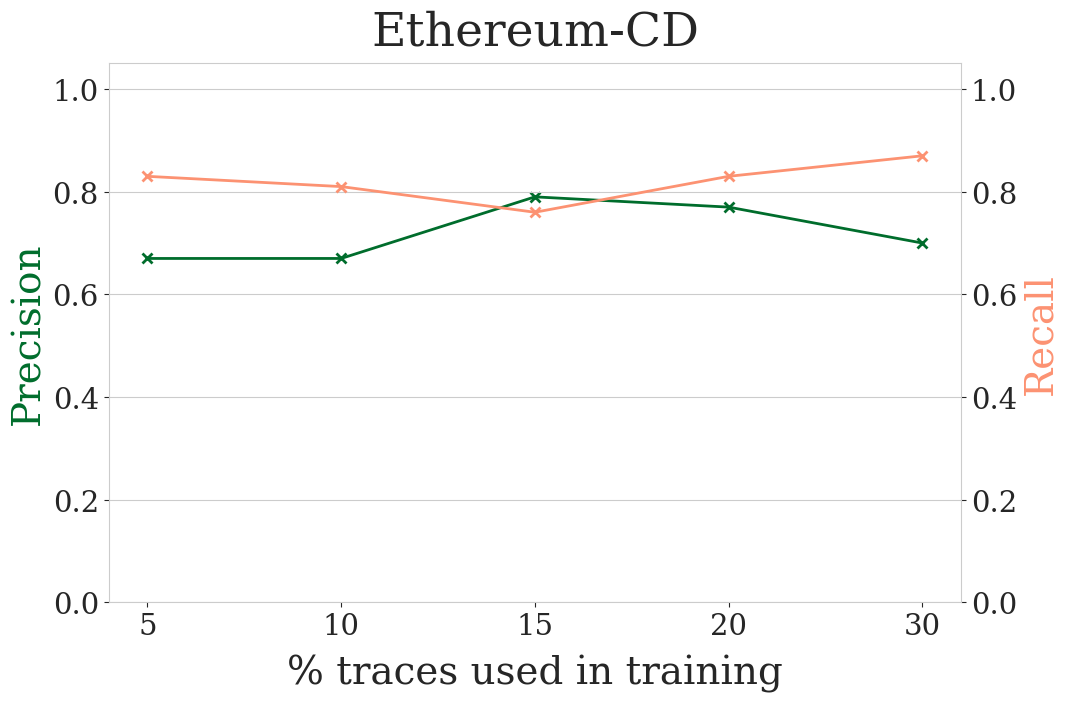
\includegraphics[scale=0.18]{6_9_eth_prec_rec_cd19_1.png}
        &
        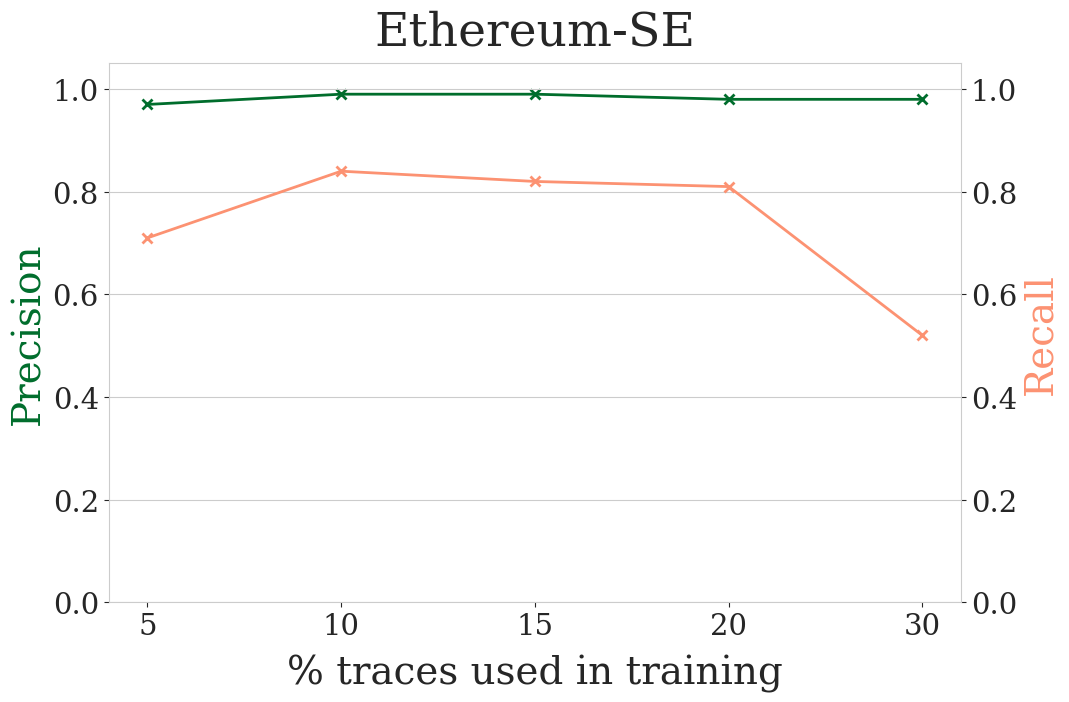
\includegraphics[scale=0.18]{6_9_eth_prec_rec_se13_1.png}
        &
        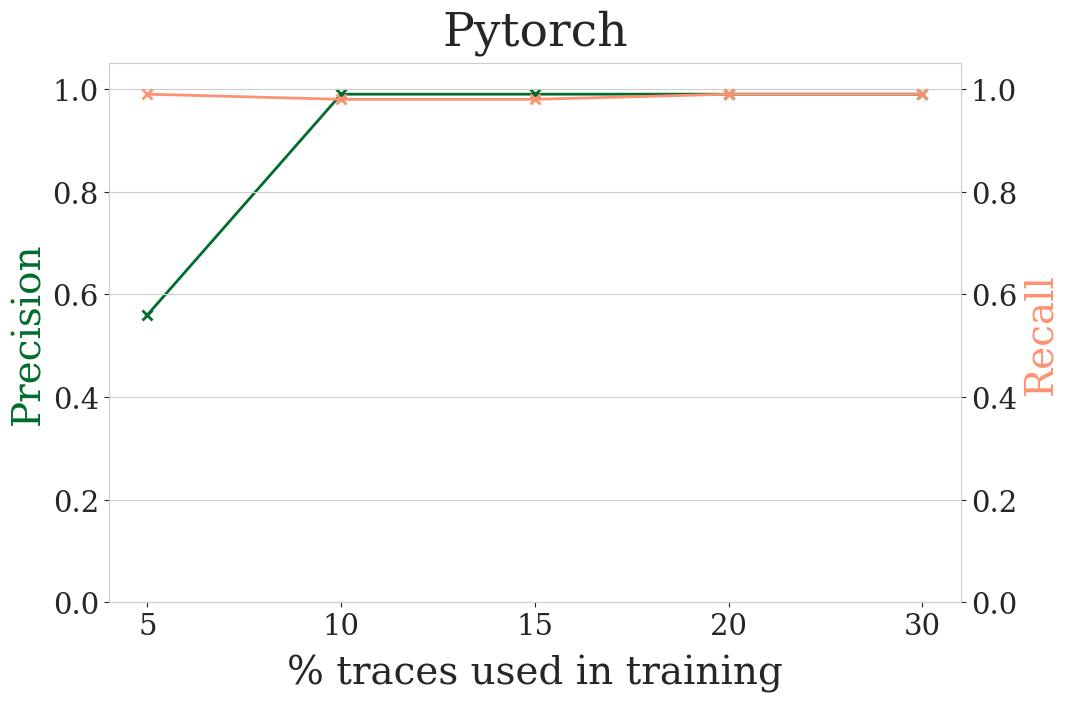
\includegraphics[scale=0.18]{6_26_pytorch_prec_rec.png}
        \\ [0.1cm]
		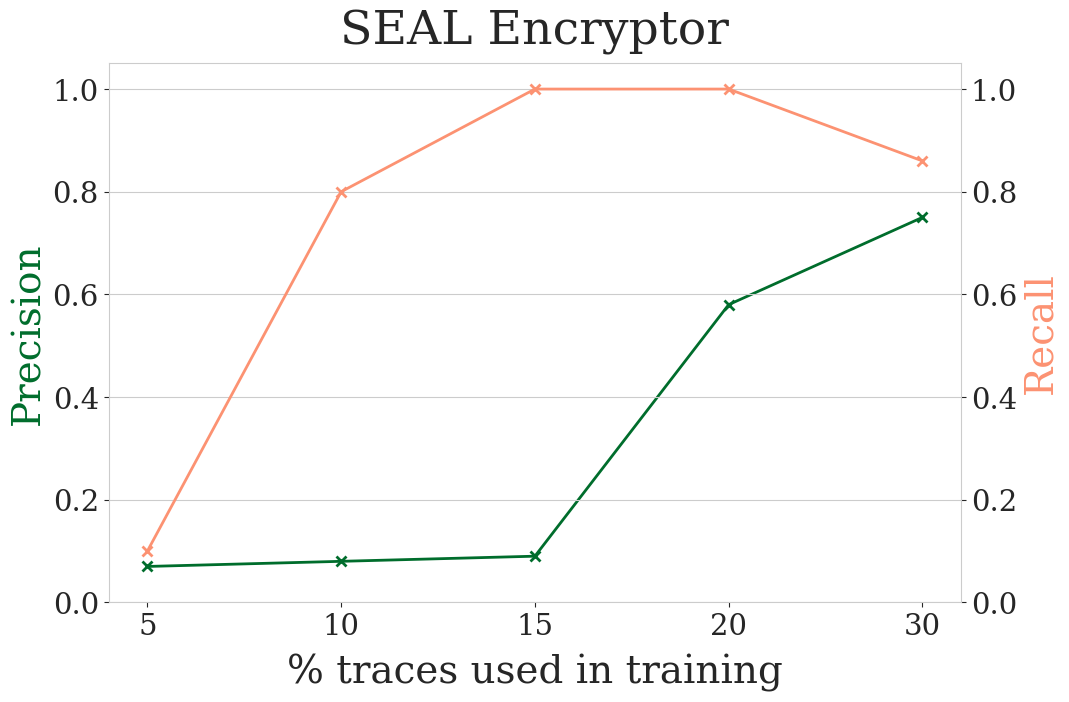
\includegraphics[scale=0.18]{6_1_sealencryptor_prec_rec.png}
		&
		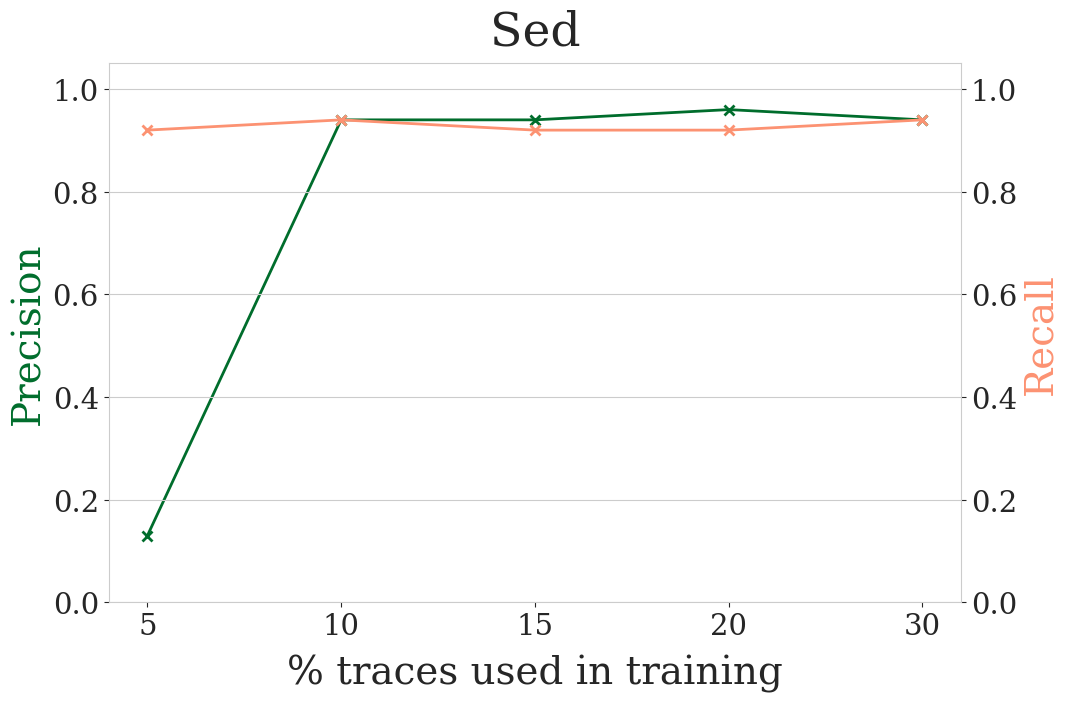
\includegraphics[scale=0.18]{6_24_sed_pr_rec.png}
%		&
%		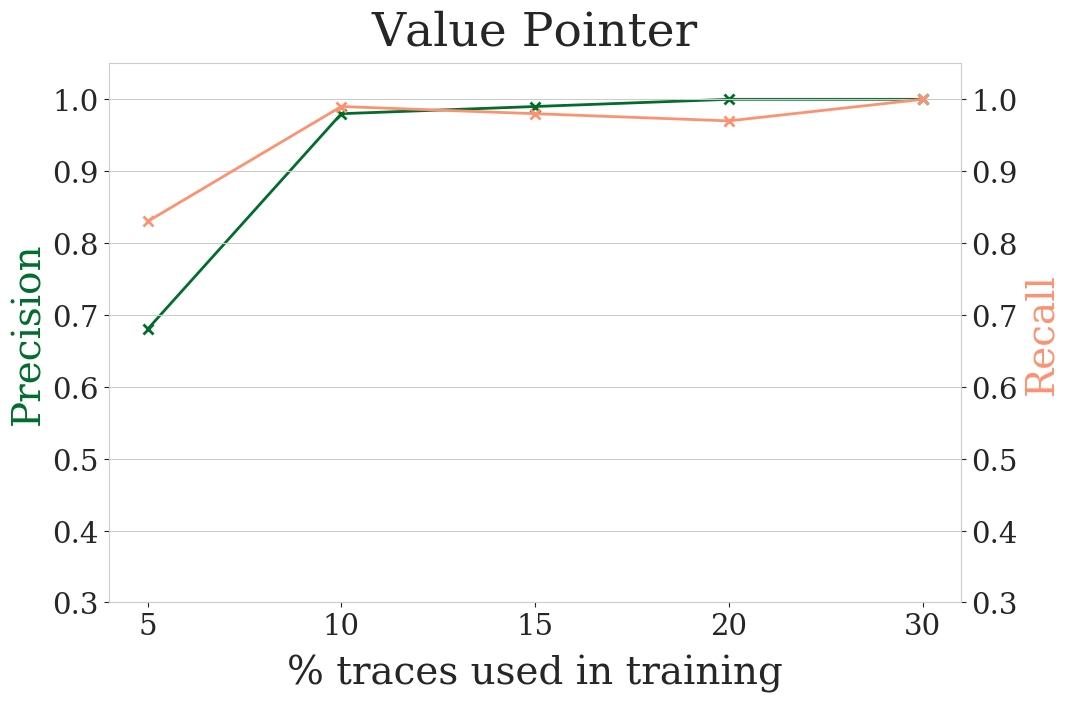
\includegraphics[scale=0.2]{6_25_valueptr_pr_rec.png}
		\\[0.1cm]
%		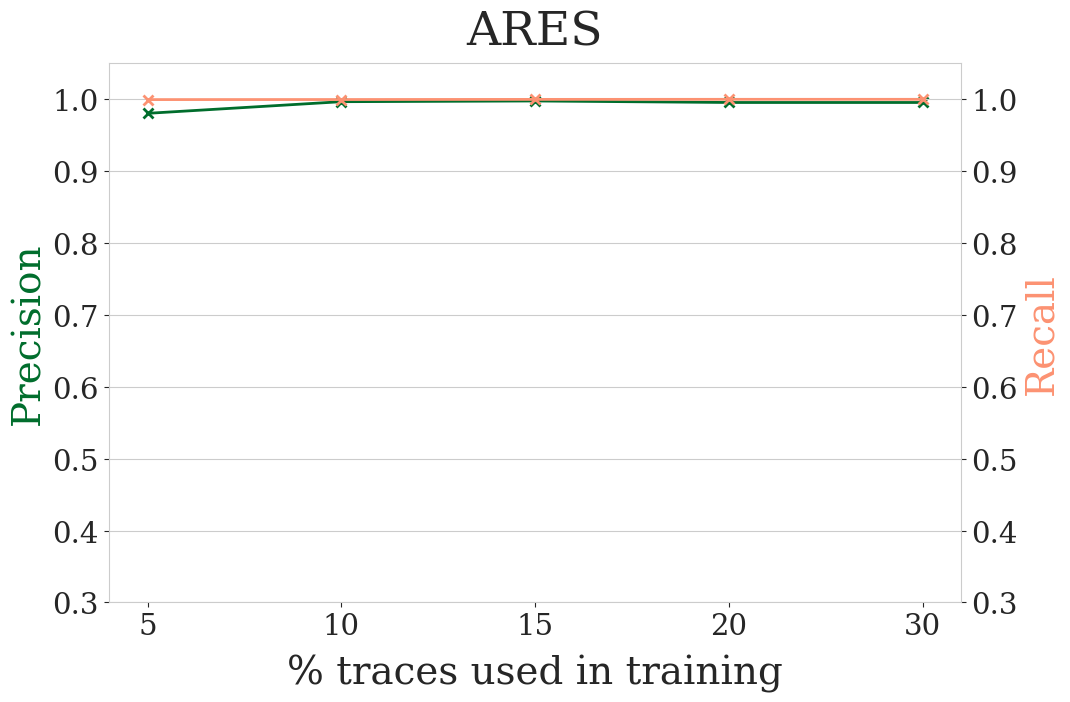
\includegraphics[scale=0.2]{6_16_fsmares_prec_rec.png}
%		&
%		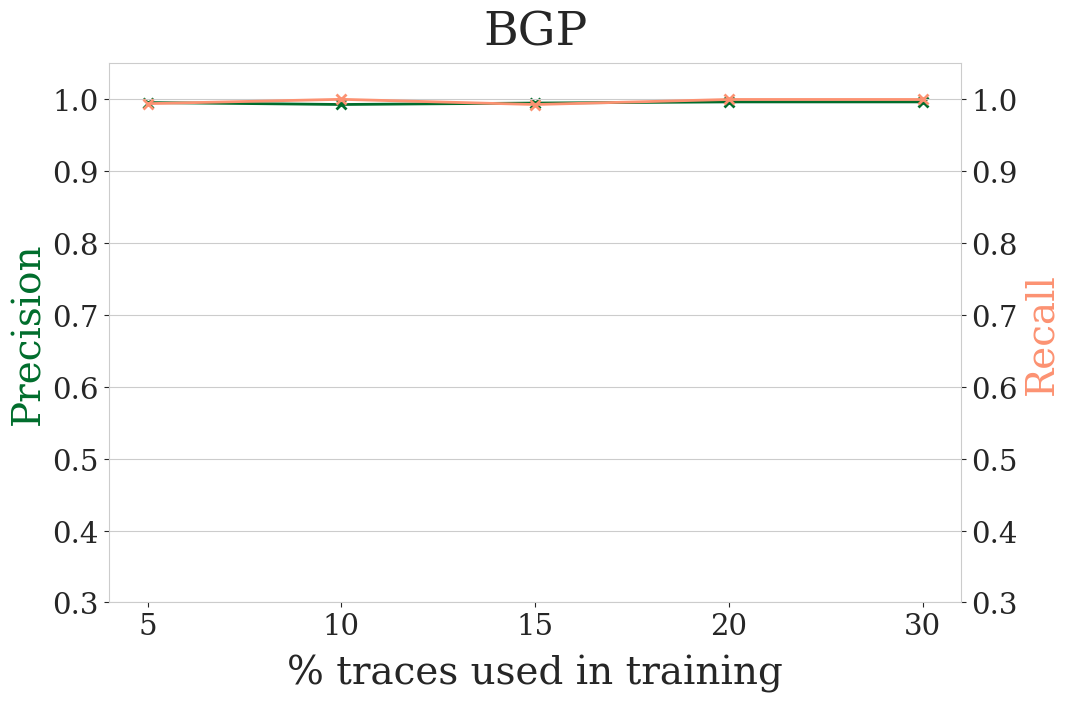
\includegraphics[scale=0.2]{6_15_fsmbgp_prec_rec.png}
%		&
%        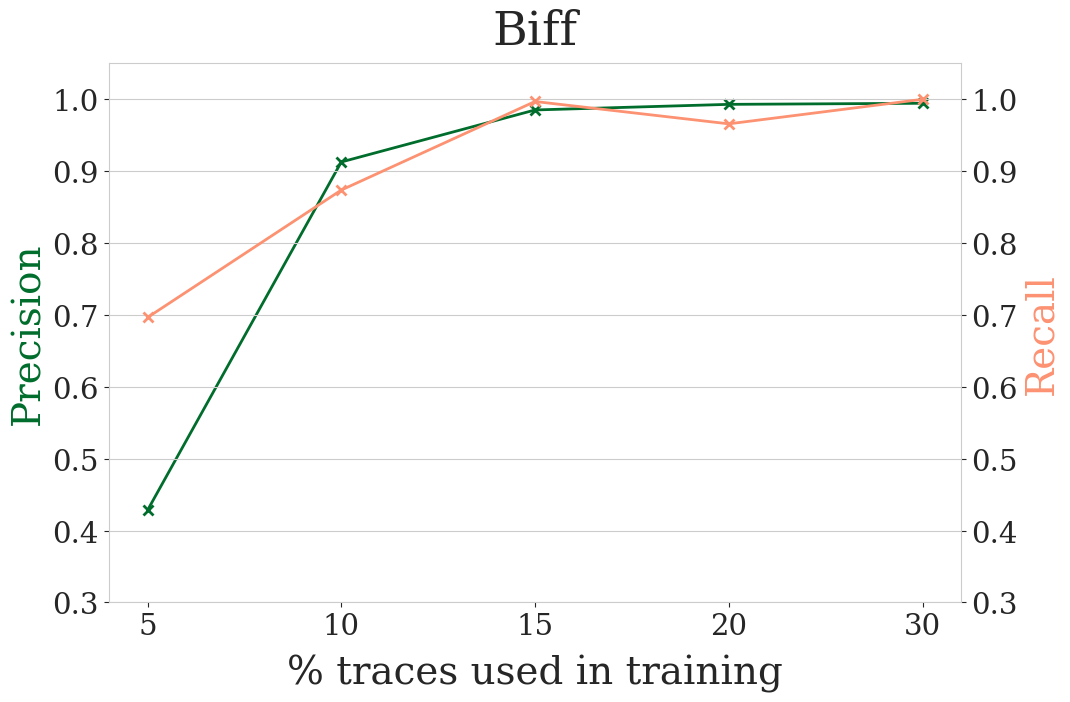
\includegraphics[scale=0.2]{6_3_fsmbiff_prec_rec.png}
%        \\[0.2cm]
%        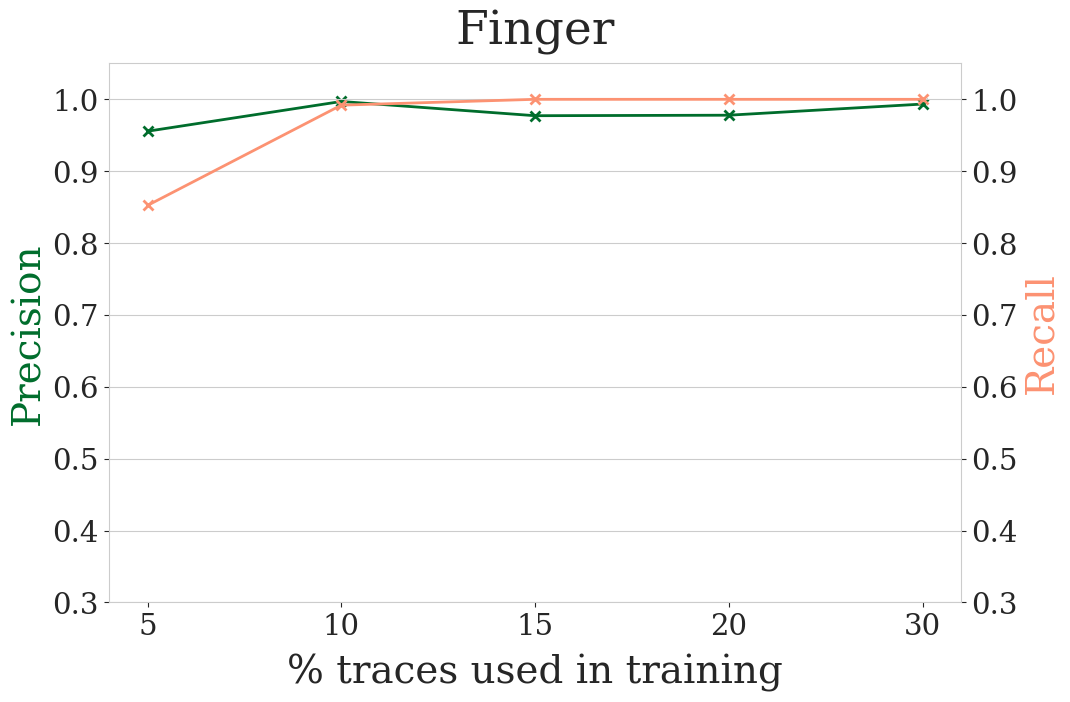
\includegraphics[scale=0.2]{6_14_fsmfinger_prec_rec.png}
%        &
%        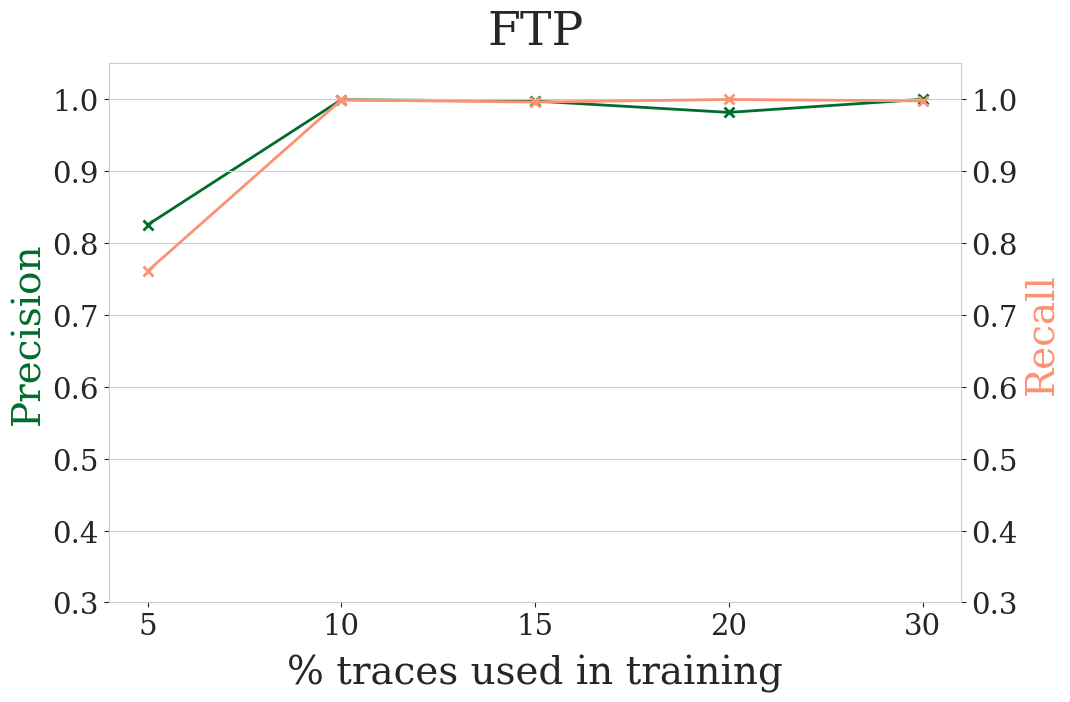
\includegraphics[scale=0.2]{6_13_fsmftp_prec_rec.png}
%        &
%        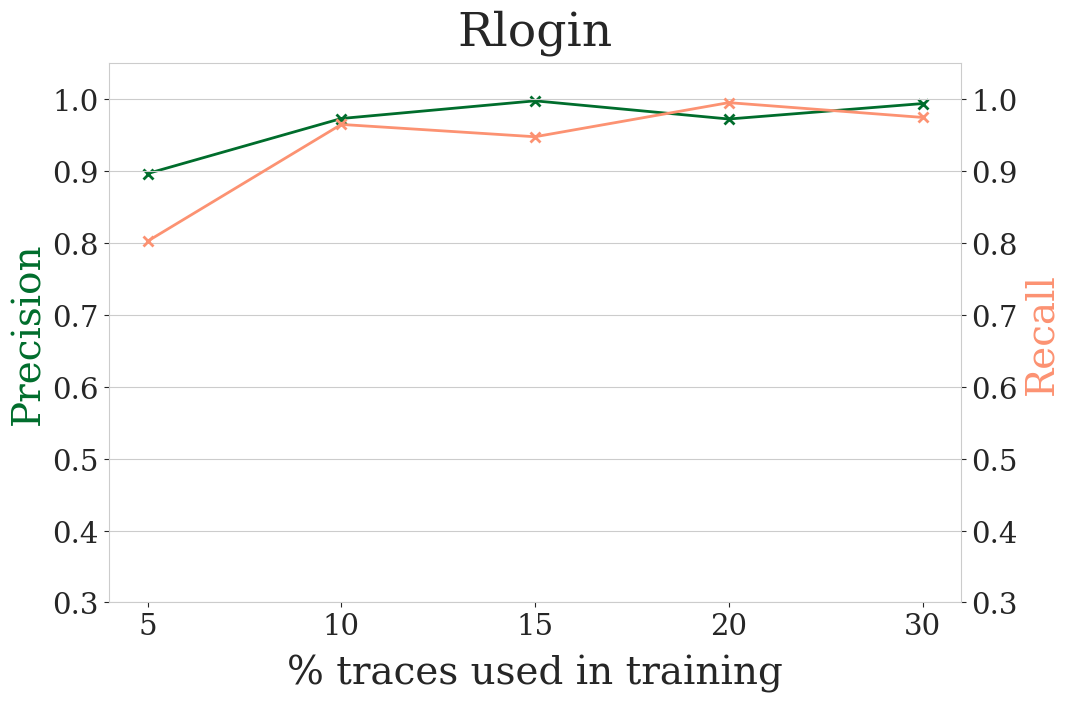
\includegraphics[scale=0.2]{6_12_fsmrlogin_prec_rec.png}
%        \\[0.2cm]
%        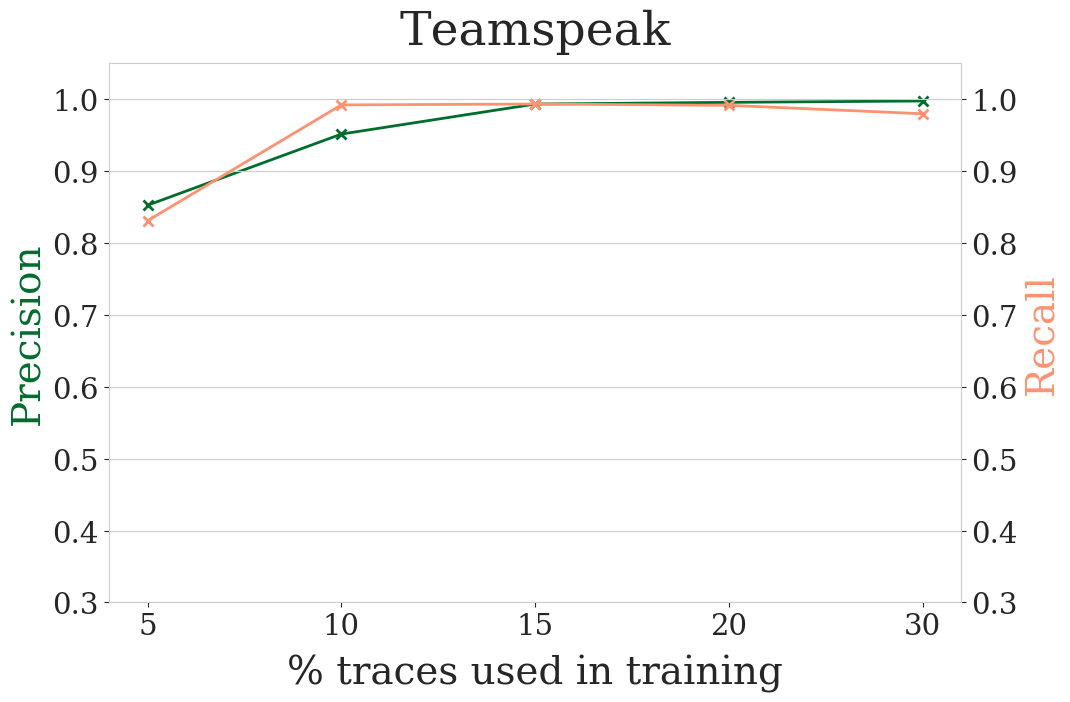
\includegraphics[scale=0.2]{6_10_fsmteamspeak_prec_rec.png}
%        &
% %       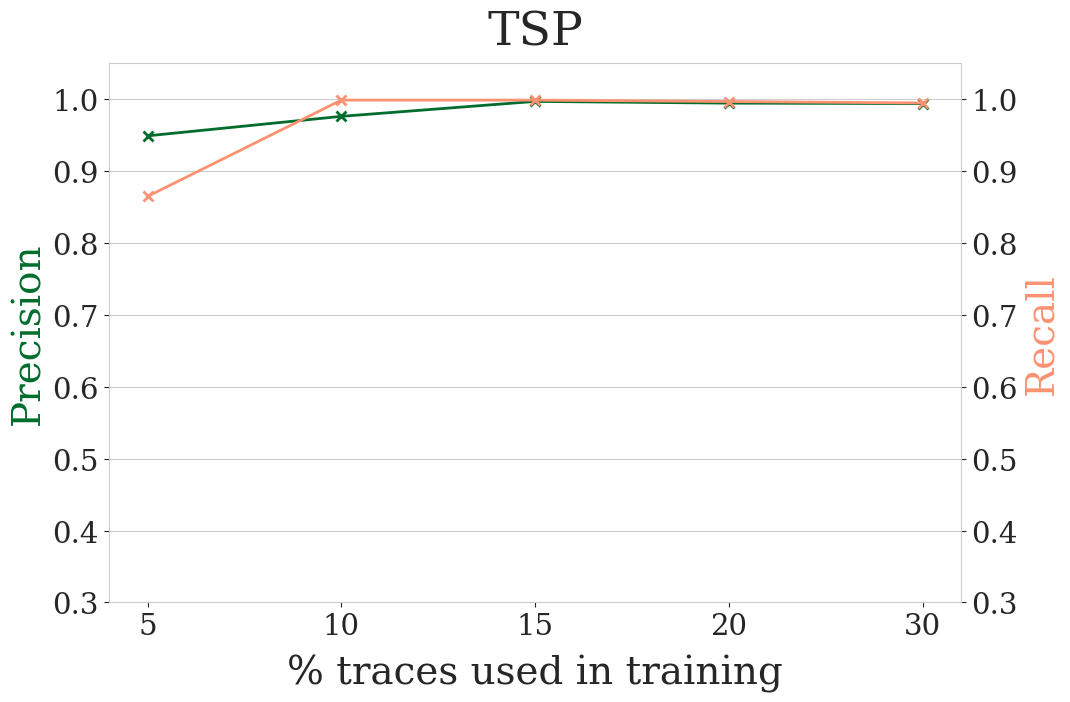
\includegraphics[scale=0.2]{6_17_fsmtsp_prec_rec.png}
% %       &
%        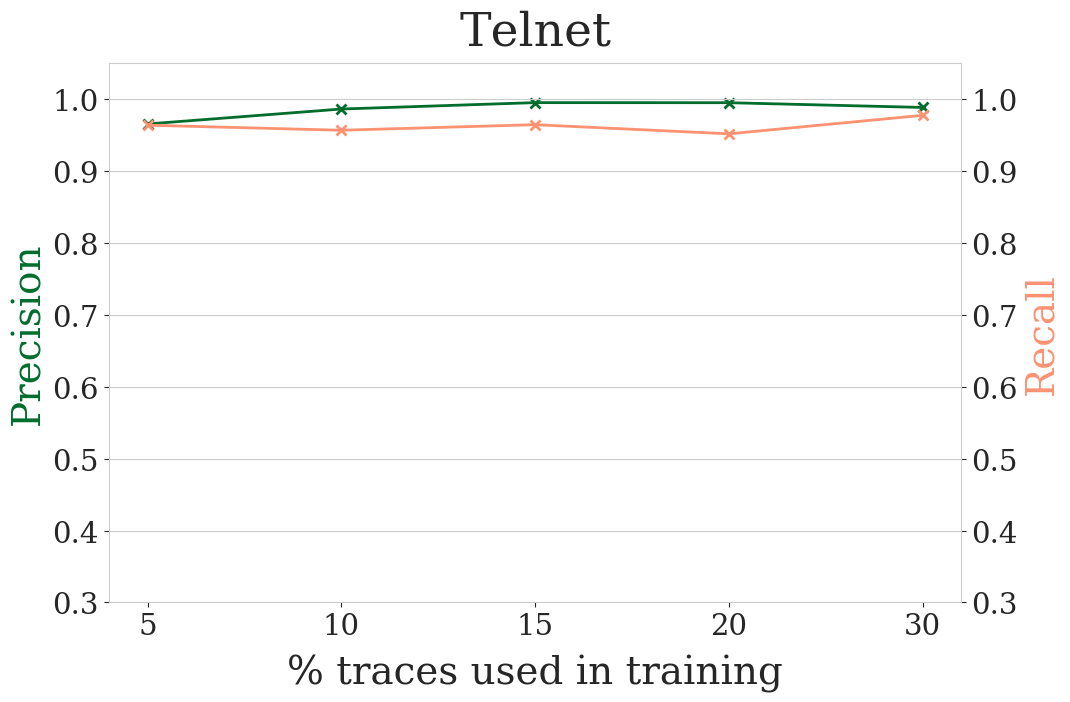
\includegraphics[scale=0.2]{6_11_fsmtelnet_prec_rec.png}
%        &
%        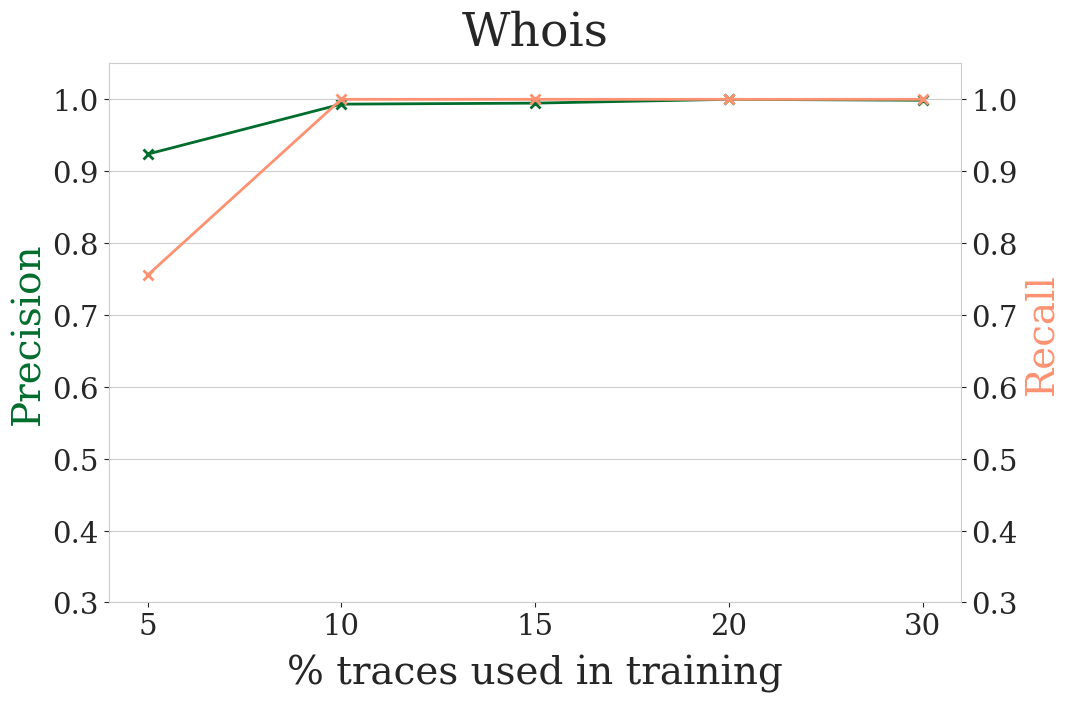
\includegraphics[scale=0.2]{6_4_fsmwhois_prec_rec.png}
%        \\ [0.2cm]
	\end{tabular}  
	\vspace{-10pt}
	\caption{Precision and recall achieved by classification model over each PUT.}
	\vspace{-5pt}
	\label{fig:precision-recall}
%	\Description[Precision and recall achieved by classification model over each PUT.]{}

\end{figure*}

%Figure~\ref{fig:precision-recall} shows fraction of traces used in training and its effect on precision and recall achieved by the classification model. 


Figure~\ref{fig:precision-recall} shows precision and recall achieved by our approach with different training set sizes.
The fraction of traces needed in training to achieve near maximal performance was 10\% to 30\% across the PUTs.
Excluding SEAL Encryptor, all the other programs only needed to be trained over 15\% of the traces to achieve near maximal performance. SEAL encryptor had very few failing traces, requiring a larger fraction of traces to get sufficient representation of failing classes during training. 
As seen in the plots in Figure~\ref{fig:precision-recall}, increasing the \% of traces used in training does not increase precision and recall for all PUTs. For instance, Pytorch and Sed observe a dramatic increase in precision and recall  when going from 5 to 10\% traces in training. Performance, however, stagnates after that point with increasing traces. With Ethereum-CD and Ethereum-SE, precision or recall becomes worse after 20\% traces. This maybe because the model is overfitting to the training traces.  
%Initially, increasing the size of training set results in better precision and recall. The extent of improvement depends on the program and execution traces. For instance, when training set size is increased from 5\% to 10\% of the overall traces, precision for \texttt{Encryptor} improves from 67\% to 95\%, while precision for \texttt{Biguint} increased steeply from 37\% to 95\%. Nevertheless, we find this observation to be true with diminishing results: after a certain point, increasing the training set size does not result in a noticeable improvement in precision and recall. We find this threshold, typically, to be between 10 to 15\%, across our subject programs.} %For the \texttt{Encryptor}, after achieving high precision with 10\% and 15\%of the traces, it drops slightly at 20\% and then goes back up to the high value at 40\%. This abnormality can occur when the model overfits to the passing traces in the training data \miltos{Is there a better way to explain this?}.  
%an average training set size of 492 traces,

It is also worth noting that the absolute size of our training set varies across subject programs. We find our approach works with training sets with as few as 3 failing traces to as many as 214. The range of passing tests in training was between 31 and 169.
\subsection{Q3. Comparison against state of art}
\label{sec:q3}

Table~\ref{tab:results} presents precision, recall, and specificity (TNR) achieved by the agglomerative hierarchical clustering proposed by Almaghairbe et al.~\cite{almaghairbe2017separating} on each of the PUTs. Comparing the precision, recall and TNR of our approach versus hierarchical clustering, we find our approach clearly outperforms the clustering approach on all but the Ethereum-CD PUT. This is because the hierarchical clustering assumption does not hold for these programs. According to this assumption, passing traces tend to be grouped in a few big clusters and failing traces are grouped into many small clusters. However, for these programs, passing traces tend to be grouped in many small clusters based on their call sequence pattern, making it hard to distinguish them from failing traces by simply comparing cluster sizes. 


With Ethereum-CD, the hierarchical clustering approach achieves precision and specificity of 100\% and a recall of 49\%. This is achieved with complete-linkage clustering, Euclidean distance and a cluster count equal to 10\% of total traces. In contrast our approach achieves a precision of 80\%, recall of 82\% and specificity of 79\%. To enable better comparison, we plot the precision-recall curve of the NN model in Figure~\ref{fig:roc} for Ethereum-CD, using 15\% of the traces in training. %\ajitha{Explain the precision recall curve and where the hierarchical clustering method falls.} %For certain programs, like the \texttt{Seal Encryptor}, the clustering approach achieves a slightly better recall ($1.0$ vs $0.98$) than our approach but the precision (of $0.5$) and TNR (of $0$) achieved with clustering are disappointing, making it unusable as it incorrectly classifies many failing and passing traces.  %The precision of $0.5$ and TNR of $0$ is, however, significantly lower than the $0.95$ precision and TNR achieved with our approach. This implies that the clustering approach does not incorrectly classify passing traces as failing, but does incorrectly classify failing traces as passing. 
%Figure~\ref{fig:roc} shows the precision and recall curve of \texttt{Ethereum-CD} when using 15\% of the traces for training. 

This curve shows the precision and recall of our trained model with respect to different values of the classification threshold.  It is clear from the plot that for the same value of recall (49\%), hierarchical clutering performs marginally better than our approach - 100\% versus 99\%. Hierarchical clustering works well over the Ethereum-CD PUT because the traces are clustered into just one big passing cluster and one failing cluster. Lack of cluster fragmentation improved accuracy of the hierarchical clustering approach. Nevertheless, our model achieves comparable performance for such traces. In addition, our model allows trade off between precision and recall by changing the classification threshold which may be driven by requirements or priorities of the use case. This tradeoff is not possible with the clustering approach. 


\begin{figure}[ht!]
\vspace{-8pt}
\centering
\includegraphics[scale=0.24]{../../figures/eth_roc_curve.png}
\vspace{-8pt}
\caption{Precision-Recall curve for \texttt{Ethereum-CD}.}
%\vspace{-20pt}
\label{fig:roc}
\vspace{-5pt}
\end{figure}
\iffalse
Overall, for 4 of the 5 subject programs, we find the clustering approach is unable to accurately distinguish failing and passing executions. This is because the hierarchical clustering assumption does not hold for these programs. According to this assumption, passing traces tend to be grouped in a few big clusters and failing traces are grouped into many small clusters. However, we find for 4 of our subject programs, passing traces also tend to be in many small clusters based on their call sequence pattern, making it hard to distinguish them from failing traces by simply comparing cluster sizes. 
However, for the Ethereum-CD program that the hierarchical clustering performs well over, the passing traces are grouped into one big cluster and the failing traces into another one. Size of the cluster of failing traces is smaller than the passing ones (despite a perfectly balanced dataset) as the technique incorrectly clusters some of the failing traces. 
\fi
%are grouped in large clusters for some programs as they have similar function call sequences as passing traces. This leads them to be incorrectly classified as passing in some cases. In addition, passing traces may also be grouped  into many small clusters when they have significant differences in method invocation sequences, especially for programs with heavy control flow, causing them to be incorrectly classified as failing in some instances. %Given the above, we also conclude that arguments and return values are vital information, therefore taking into account only callee name sequences significantly hinders classification accuracy.

%as the our approach has significantly higher accuracy than the clustering approach in correctly identifying and classifying both failing and passing traces. 
%Discuss each program and outliers. Average difference?

\iffalse
\textcolor{red}{\subsection{Q4. Generalisation}
\label{sec:q4}
In this research question, we conduct an initial exploration into the ambitious possibility of using a model, trained using traces from one subject program, to classify traces from other programs in the same application domain. We use FSMs from the network protocol domain to evaluate this possibility. Figures~\ref{biff_cross} and~\ref{whois_cross} represent precision and recall achieved by models trained using traces from \texttt{Biff} protocol and \texttt{Whois} protocol, respectively, to classify traces produced by other FSMs.
We find that the model trained using traces from \texttt{Biff} achieves high accuracy over the \texttt{Ares} protocol with precision and recall close to 1.0, and reasonable
precision ($ > 0.8$) for \texttt{BGP, FTP, Rlogin, Teamspeak, Whois} protocols. Lowest precision ($0.17$) was observed with \texttt{Telnet}. Average precision achieved in classifying traces from unseen FSMs was $0.79$.
Recall achieved by the model is lower than precision indicating that the model missed identifying failing traces in each of these protocols.  
Overall, the model trained with \texttt{Biff} traces was successful in identifying failing traces in other FSMs that have similar patterns to \texttt{Biff}. Failing traces with differing patterns were missed.  
We confirmed this observation by checking results from the \texttt{Whois} model. Although precision and recall numbers are different from the \texttt{Biff} model, the reasoning for classification success was the same - extent of similarity in execution patterns between FSMs.
%Although precision is higher, in general, than the average precision of the \texttt{Biff} model, the reasoning for higher recall was the same - extent of similarity in execution patterns between FSMs.
With the current approach, we find there is scope to generalise a classification model from a single FSM to multiple FSMs in the networking domain. However, achieving high accuracies with generalisation is a difficult problem and we plan to take small, definitive steps towards addressing this challenge in the future. As a next step, we will explore tuning the classification model from an individual FSM with sample traces from other FSMs to improve generalisation performance.  %and we believe that fine tuning or techniques like transfer learning will help 
}


\begin{figure}[ht!]
\centering
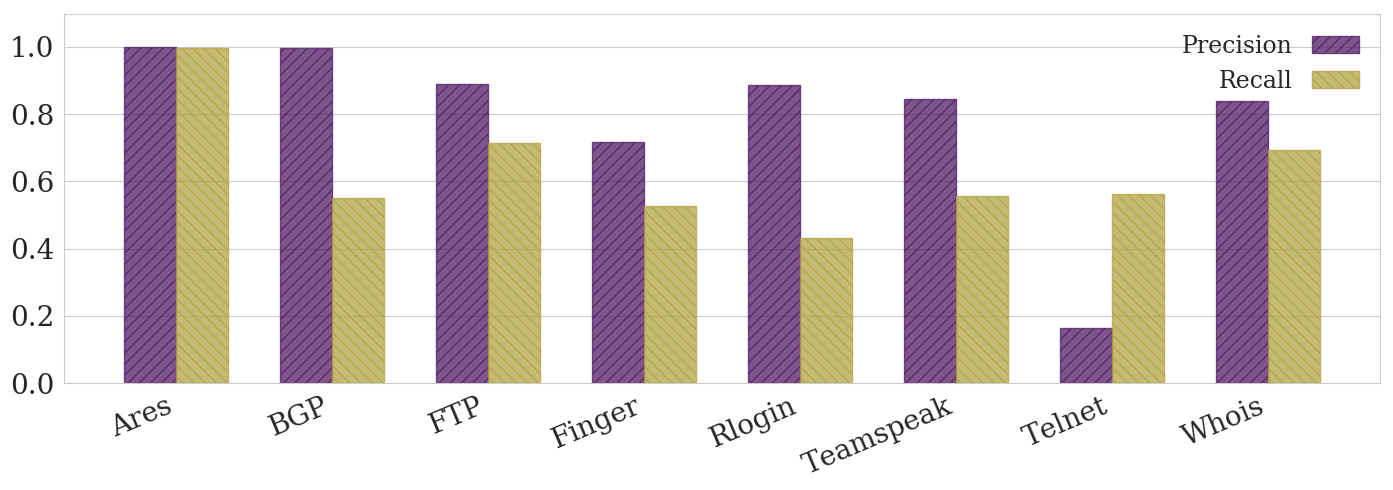
\includegraphics[scale=0.25]{6_5_biff_cross.png}
\vspace{-10pt}
\caption{\texttt{Biff} trained model - Precision and recall for unseen fsms.}
\Description[\texttt{Biff} trained model - Precision and recall for unseen fsms.]{}
\vspace{-10pt}
\label{biff_cross}
\end{figure}

\begin{figure}[ht!]
\centering
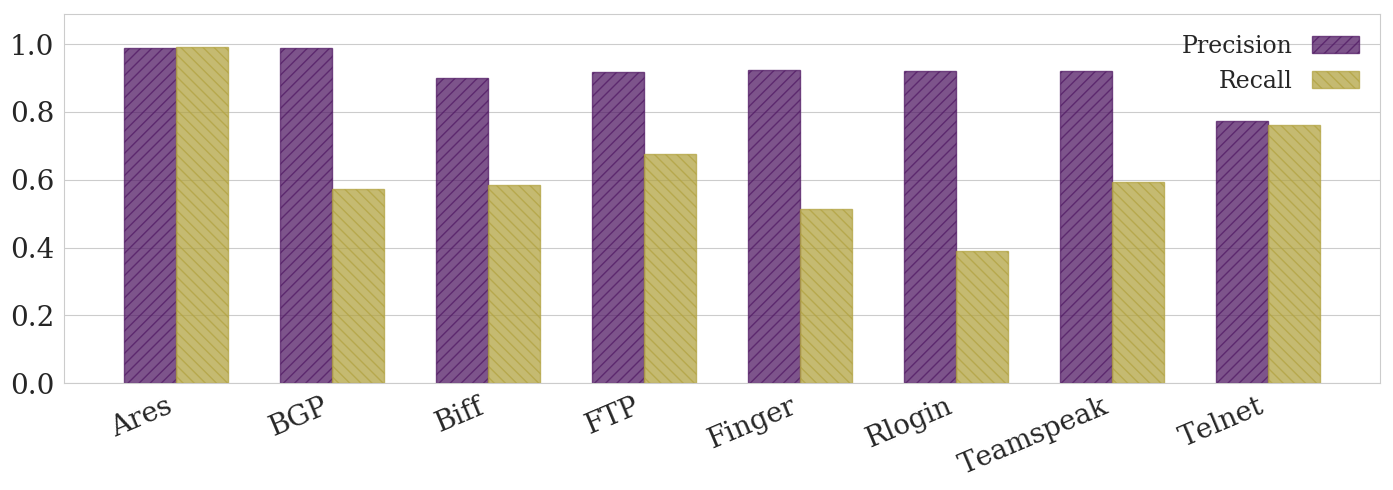
\includegraphics[scale=0.25]{6_6_whois_cross.png}
\vspace{-10pt}
\caption{\texttt{Whois} trained model - Precision and recall for unseen fsms.}
\Description[\texttt{Whois} trained model - Precision and recall for unseen fsms.]{}
\vspace{-15pt}
\label{whois_cross}
\end{figure}
\fi
\subsection{Threats to Validity}
\label{sec:threats}
We see three threats to validity of our
experiment based on the selection of subject programs and associated tests. 

%The subject programs in our experiment, expected output is provided with the tests and that is used for labelling the traces. 
%If the tests fo not specify the expected outputs, then a developer or expert would have to manually label the traces used in training, which is 
%a small fraction of the total traces that they would otherwise have to label. 
First, PUTs for 3 out of the 4 subject programs in our experiment were generated by seeding faults into a reference implementation. A reference implementation with only passing tests is not suitable for evaluating our approach.  To address this, we generated a faulty implementation and ran the original tests through the PUT to gather both passing and failing traces.  
%To avoid an imbalanced training set, we generated failing execution traces using seeded faults representing common bug patterns~\cite{jia2011analysis, pradel2018deepbugs}. %mutating passing test inputs and checking if they cause the actual output to differ from the expected output. 
It is possible using real faults in place of seeded faults may lead to
different results. However, Andrews et al. have shown the use of seeded faults leads to conclusions
similar to those obtained using real faults~\cite{andrews2006using, Do1707670}. 
For one of the subject programs, Sed,  we did not artificially seed faults, but instead used the existing implementation as it was accompanied by both passing and failing tests. % which helps mitigate this threat. 

Second, the number of tests that accompanied our subject programs was not very large, ranging from 132 to 2254 tests. The NN models in our experiments produced good performance with small to medium sized test suites that may be automatically or manually generated. Our approach is constrained by the amount of training data and not by the size of the test suite. As a result for programs accompanied by large test suites, the NN model will need a larger training set (fraction of traces to be used in training might still be 15\%). Nevertheless, the labelling effort for a fraction of the tests in our approach is still less than the current practise of labelling all the tests. 
%Although our experiment lacks subject programs with a large test suite, we believe achieving good performance over approach is well suited to NN models for programs with larger test sets will perform  
%These programs did not have adequate tests that can be used for training and evaluation. 

%This was done to increase the size of data set available training and evaluation. 

Finally, we conducted our study on subject programs from 4 different application domains which is not representative of all application domains. %The NN model in our approach is learned and trained for each subject program and used to classify traces for just that program. 
Given that our approach has no domain specific constraints, we believe it will be widely applicable. %owill result in high accuracy test classification for subject programs in other domains as well. 
%We believe our approach for learnign a model to classify traces will work well for programs in other domains as well as there is no 
%We believe these systems are representative of the class of systems in which we are interested, and our
%results are thus generalizable to other systems in the domain.


\iffalse
Another threat to external validity relates
to the test suites used in our study. 
We used existing test suites for the SIR programs and randomly generated test suites that are controlled for 
test suite size for the EEMBC programs and LLVM Symbolizer. 
We cannot claim that the test
suites we used are necessarily representative of all possible
test suites.
Additional
research is needed to assess the performance of locality ordering with
different test generation frameworks
and with hand-written tests.
\fi

\iffalse

\begin{table}[]
\centering
%\iffalse
\begin{tabular}{|c|c|c|c|c|}
	\hline
	Trace section omitted   & {Precision} & {Recall} & TNR\\ 
	\hline \hline
	Function names  & 0.49 & 0.98 & 0.02 \\ \hline 
	Return values & 0.50  & 0.94 & 0.07 \\ \hline
	Arguments & 0.52  & 0.91 & 0.36 \\ \hline
	Half the \#trace lines & 0.70 & 0.86 & 0.63 \\ \hline 
\end{tabular}
%\fi
\caption{Precision and Recall of models trained with traces omitting certain information for \texttt{Ethereum}. }
\label{tab:ethereum_removed_trace}
\end{table}

\begin{table}[]
\centering
%\iffalse
\begin{tabular}{|c|c|c|c|c|}
	\hline
	Trace section omitted   & {Precision} & {Recall} & TNR\\ 
	\hline \hline
	Function names  & 0.92 & 0.14 & 0.98 \\ \hline 
	Return values & 0.79  & 0.98 & 0.74 \\ \hline
	Arguments & 0.70  & 0.98 & 0.59 \\ \hline
	Half the \#trace lines & 0.72 & 1.0 & 0.58 \\ \hline 
\end{tabular}
%\fi
\caption{Precision and Recall of models trained with traces omitting certain information for \texttt{Encryptor}. }
\label{tab:encryptor_removed_trace}
\end{table}

\begin{table}[]
\centering
%\iffalse
\begin{tabular}{|c|c|c|c|c|}
	\hline
	Trace section omitted   & {Precision} & {Recall} & TNR\\ 
	\hline \hline
	Function names  & 0.95 & 0.58 & 0.97 \\ \hline 
	Return values & 0.97  & 0.94 & 0.97 \\ \hline
	Arguments & 0.90  & 0.88 & 0.91 \\ \hline
	Half the \#trace lines & 0.81 & 0.90 & 0.79 \\ \hline 
\end{tabular}
%\fi
\caption{Precision and Recall of models trained with traces omitting certain information for \texttt{Biguint}. }
\label{tab:biguint_removed_trace}
\end{table}

\begin{table}[]
\centering
%\iffalse
\begin{tabular}{|c|c|c|c|c|}
	\hline
	Trace section omitted   & {Precision} & {Recall} & TNR\\ 
	\hline \hline
	Function names  & 0.62 & 0.86 & 0.37 \\ \hline 
	Return values & 0.47  & 1.0 & 0.0 \\ \hline
	Arguments & 0.52  & 0.96 & 0.04 \\ \hline
	Half the \#trace lines & 0.47 & 1.0 & 0.0 \\ \hline 
\end{tabular}
%\fi
\caption{Precision and Recall of models trained with traces omitting certain information for \texttt{Value pointer}. }
\label{tab:valueptr_removed_trace}
\end{table}



\begin{table}[]
\centering
%\iffalse
\begin{tabular}{|c|c|c|c|c|}
	\hline
	Trace section omitted   & {Precision} & {Recall} & TNR\\ 
	\hline \hline
	Function names  & 0.11 & 1.0 & 0.02 \\ \hline 
	Return values & 0.20  & 0.24 & 0.89 \\ \hline
	Arguments & 0.67  & 0.08 & 0.99 \\ \hline
	Half the \#trace lines & 1.0 & 0.08 & 1.0 \\ \hline 
\end{tabular}
%\fi
\caption{Precision and Recall of models trained with traces omitting certain information for \texttt{Sed}. }
\label{tab:sed_removed_trace}
\end{table}


\begin{table}[]
\centering
%\iffalse
\begin{tabular}{|c|c|c|c|c|}
	\hline
	Trace section omitted   & {Precision} & {Recall} & TNR\\ 
	\hline \hline
	Function names  & 0.96 & 0.98 & 0.95 \\ \hline 
	Return values & 0.95  & 0.99 & 0.75 \\ \hline
	Arguments & 0.93  & 0.96 & 0.68 \\ \hline
	Half the \#trace lines & 0.99 & 0.99 & 0.79 \\ \hline
	Global state & 0.95 & 0.96 & 0.97 \\ \hline 
\end{tabular}
%\fi
\caption{Precision and Recall of models trained with traces omitting certain information for \texttt{Ares} protocol. }
\label{tab:ares_removed_trace}
\end{table}


\begin{table}[]
\centering
%\iffalse
\begin{tabular}{|c|c|c|c|c|}
	\hline
	Trace section omitted   & {Precision} & {Recall} & TNR\\ 
	\hline \hline
	Function names  & 0.99 & 0.98 & 0.98 \\ \hline 
	Return values & 0.98 & 0.99 & 0.98 \\ \hline
	Arguments & 0.97  & 0.97 & 0.97 \\ \hline
	Half the \#trace lines & 0.62 & 0.84 & 0.48 \\ \hline
	Global state & 0.62 & 0.87 & 0.47 \\ \hline
\end{tabular}
%\fi
\caption{Precision and Recall of models trained with traces omitting certain information for \texttt{BGP} protocol. }
\label{tab:bgp_removed_trace}
\end{table}



\begin{table}[]
\centering
%\iffalse
\begin{tabular}{|c|c|c|c|c|}
	\hline
	Trace section omitted   & {Precision} & {Recall} & TNR\\ 
	\hline \hline
	Function names  & 0.58 & 0.84 & 0.41 \\ \hline 
	Return values & 0.56 & 0.92 & 0.35 \\ \hline
	Arguments & 0.51  & 0.64 & 0.40 \\ \hline
	Half the \#trace lines & 0.51 & 0.81 & 0.23 \\ \hline
	Global state & 0.62 & 0.76 & 0.55 \\ \hline
\end{tabular}
%\fi
\caption{Precision and Recall of models trained with traces omitting certain information for \texttt{Biff} protocol. }
\label{tab:biff_removed_trace}
\end{table}


\begin{table}[]
\centering
%\iffalse
\begin{tabular}{|c|c|c|c|c|}
	\hline
	Trace section omitted   & {Precision} & {Recall} & TNR\\ 
	\hline \hline
	Function names  & 0.99 & 0.95 & 0.99 \\ \hline 
	Return values & 0.98 & 0.97 & 0.99 \\ \hline
	Arguments & 0.52  & 0.19 & 0.88 \\ \hline
	Half the \#trace lines & 0.49 & 0.60 & 0.59 \\ \hline
	Global state & 0.97 & 0.94 & 0.97 \\ \hline
\end{tabular}
%\fi
\caption{Precision and Recall of models trained with traces omitting certain information for \texttt{Finger} protocol. }
\label{tab:finger_removed_trace}
\end{table}


\begin{table}[]
\centering
%\iffalse
\begin{tabular}{|c|c|c|c|c|}
	\hline
	Trace section omitted   & {Precision} & {Recall} & TNR\\ 
	\hline \hline
	Function names  & 0.99 & 0.99 & 0.98 \\ \hline 
	Return values & 0.97 & 0.97 & 0.98 \\ \hline
	Arguments & 0.88  & 0.93 & 0.84 \\ \hline
	Half the \#trace lines & 0.71 & 0.91 & 0.52 \\ \hline
	Global state & 0.96 & 0.96 & 0.98 \\ \hline 
\end{tabular}
%\fi
\caption{Precision and Recall of models trained with traces omitting certain information for \texttt{FTP} protocol. }
\label{tab:ftp_removed_trace}
\end{table}

\begin{table}[]
\centering
%\iffalse
\begin{tabular}{|c|c|c|c|c|}
	\hline
	Trace section omitted   & {Precision} & {Recall} & TNR\\ 
	\hline \hline
	Function names  & 0.95 & 0.96 & 0.96 \\ \hline 
	Return values & 1.0 & 0.92 & 1.0 \\ \hline
	Arguments & 0.85  & 0.91 & 0.94 \\ \hline
	Half the \#trace lines & 0.93 & 0.93 & 0.97 \\ \hline
	Global state & 0.92 & 0.95 & 0.92 \\ \hline 
\end{tabular}
%\fi
\caption{Precision and Recall of models trained with traces omitting certain information for \texttt{Rlogin} protocol. }
\label{tab:rlogin_removed_trace}
\end{table}

\begin{table}[]
\centering
%\iffalse
\begin{tabular}{|c|c|c|c|c|}
	\hline
	Trace section omitted   & {Precision} & {Recall} & TNR\\ 
	\hline \hline
	Function names  & 0.91 & 0.97 & 0.91 \\ \hline 
	Return values & 0.94 & 0.98 & 0.94 \\ \hline
	Arguments & 0.77  & 0.86 & 0.77 \\ \hline
	Half the \#trace lines & 0.93 & 0.93 & 0.97 \\ \hline
	Global state & 0.90 & 0.93 & 0.91 \\ \hline 
\end{tabular}
%\fi
\caption{Precision and Recall of models trained with traces omitting certain information for \texttt{Teamspeak} protocol. }
\label{tab:teamspeak_removed_trace}
\end{table}


\begin{table}[]
\centering
%\iffalse
\begin{tabular}{|c|c|c|c|c|}
	\hline
	Trace section omitted   & {Precision} & {Recall} & TNR\\ 
	\hline \hline
	Function names  & 0.88 & 1.0 & 0.49 \\ \hline 
	Return values & 0.82 & 1.0 & 0.25 \\ \hline
	Arguments & 0.76  & 1.0 & 0.0 \\ \hline
	Half the \#trace lines & 0.75 & 0.93 & 0.0 \\ \hline
	Global state & 0.88 & 1.0 & 0.49 \\ \hline 
\end{tabular}
%\fi
\caption{Precision and Recall of models trained with traces omitting certain information for \texttt{Telnet} protocol. }
\label{tab:telnet_removed_trace}
\end{table}
%
\begin{table}[]
\centering
%\iffalse
\begin{tabular}{|c|c|c|c|c|}
	\hline
	Trace section omitted   & {Precision} & {Recall} & TNR\\ 
	\hline \hline
	Function names  & 0.96 & 0.97 & 0.96 \\ \hline 
	Return values & 0.94 & 0.97 & 0.96 \\ \hline
	Arguments & 0.94  & 0.97 & 0.96 \\ \hline
	Half the \#trace lines & 0.85 & 0.94 & 0.90 \\ \hline
	Global state & 0.93 & 0.95 & 0.92 \\ \hline 
\end{tabular}
%\fi
\caption{Precision and Recall of models trained with traces omitting certain information for \texttt{TSP} protocol. }
\label{tab:tsp_removed_trace}
\end{table}

\begin{table}[]
\centering
%\iffalse
\begin{tabular}{|c|c|c|c|c|}
	\hline
	Trace section omitted   & {Precision} & {Recall} & TNR\\ 
	\hline \hline
	Function names  & 0.96 & 0.96 & 0.96 \\ \hline 
	Return values & 0.96 & 0.96 & 0.96 \\ \hline
	Arguments & 0.72  & 0.75 & 0.73 \\ \hline
	Half the \#trace lines & 0.58 & 0.61 & 0.60 \\ \hline
	Global state & 0.96 & 0.96 & 0.96 \\ \hline 
\end{tabular}
%\fi
\caption{Precision and Recall of models trained with traces omitting certain information for \texttt{Whois} protocol. }
\label{tab:whois_removed_trace}
\end{table}

\fi

\iffalse
\begin{table*}[]
\centering
\small
\begin{tabular}{|l|l|l|l|l|l@{\hskip 5mm}|l|l|l|}
	\hline
	Mutation & CD1 & CD9 & CD10 & CD19 & CD20 \\ 
	\hline
	5\% & 0.65, 0.91, 0.51 & 0.99, 0.63, 0.99 & 0.86, 0.70, 0.88 & 0.67, 0.83, 0.59 & 0.64, 0.93, 0.50  \\ \hline
	10\% & 0.92, 0.70, 0.94 & 0.70, 0.94, 0.60 & 0.64, 0.81, 0.51 & 0.67, 0.81, 0.61 & 0.76, 0.84, 0.73 \\ \hline
	15\% & 0.78, 0.74, 0.80 & 0.74, 0.82, 0.74 & 0.84, 0.77, 0.86 & 0.79, 0.76, 0.79 & 0.76, 0.73, 0.77 \\ \hline
	20\% & 0.83, 0.80, 0.83 & 0.89, 0.72, 0.91 & 0.82, 0.67, 0.86 & 0.77, 0.83, 0.74 & 0.80, 0.80, 0.80 \\ \hline
	30\% & 0.86, 0.71, 0.88 & 0.91, 0.74, 0.92 & 0.77, 0.81, 0.76 & 0.70, 0.87, 0.64 & 0.75, 0.83, 0.72 \\
	\hline
\end{tabular}
\caption{Pr, Rec, TNR for each ethereum mutation with respect to the size of training set (\textcolor{red}{Ratio in these mutations: 1127 pass, 1127 fail})}
\vspace{-20pt}
\label{tab:eth-1}
\end{table*}



\begin{table*}[]
\centering
\small
\begin{tabular}{|l|l|l|l|l|l|l@{\hskip 5mm}|l|l|l|}
	\hline
	Mutation & SE13 (92p, 2162f) & SE16 (1334p, 920f) & SE17 (1334p, 920f) & SE18 (1426p, 828f) \\ 
	\hline
	5\% & 0.97, 0.71, 0.59 & 1, 1, 1 & 0.99, 0.99, 0.99 & 0.88, 0.97, 0.92 \\ \hline
	10\% & 0.99, 0.84, 0.73 & 1, 1, 1 & 0.97, 0.97, 0.98 & 0.90, 0.94, 0.94 \\ \hline
	15\% & 0.99, 0.82, 0.86 & 1, 1, 1 & 0.96, 0.96, 0.97 & 0.86, 0.97, 0.91 \\ \hline
	20\% & 0.98, 0.81, 0.58 & 1, 1, 1 & 0.92, 0.93, 0.94 & 0.89, 0.91, 0.94 \\ \hline
	30\% & 0.98, 0.52, 0.75 & 1, 1, 1 & 0.96, 0.97, 0.98 & 0.99, 0.99, 0.99 \\ \hline
\end{tabular}
\caption{Pr, Rec, TNR for each ethereum mutation with respect to the size of training set, with ratio embedded in title}
\vspace{-20pt}
\label{tab:eth-2}
\end{table*}


\begin{table*}[]
\centering
\small
\begin{tabular}{|l|l|l|l|l|l|l@{\hskip 5mm}|l|l|l|}
	\hline
	Mutation & Func names & Return val & Arguments & Half trace \\ 
	\hline
	5\% & 0.70, 0.72, 0.69 & 0.72, 0.73, 0.72 & 0.52, 0.82, 0.26 & 0.69, 0.85, 0.61 \\ \hline
	10\% & 0.74, 0.76, 0.74 & 0.71, 0.92, 0.64 & 0.59, 0.82, 0.44 & 0.82, 0.80, 0.83 \\ \hline
	15\% & 0.75, 0.85, 0.70 & 0.81, 0.72, 0.84 & 0.66, 0.83, 0.56 & 0.73, 0.77, 0.71 \\ \hline
	20\% & 0.94, 0.64, 0.97 & 0.50, 0.89, 0.11 & 0.79, 0.69, 0.82 & 0.94, 0.68, 0.96 \\ \hline
	30\% & 0.92, 0.66, 0.94 & 0.82, 0.81, 0.81 & 0.71, 0.92, 0.62 & 0.89, 0.70, 0.91 \\ \hline
\end{tabular}
\caption{Pr, Rec, TNR for CD1 mutation, ablation study}
\vspace{-20pt}
\label{tab:eth-3}
\end{table*}


\begin{table*}[]
\centering
\small
\begin{tabular}{|l|l|l|l|l|l|l@{\hskip 5mm}|l|l|l|}
	\hline
	Mutation & Func names & Return val & Arguments & Half trace \\ 
	\hline
	10\% & 0.63, 0.64, 0.62 & 0.68, 0.87, 0.60 & 0.54, 0.78, 0.35 & 0.81, 0.83, 0.80 \\ \hline
\end{tabular}
\caption{Pr, Rec, TNR for CD19 mutation, ablation study}
\vspace{-20pt}
\label{tab:eth-4}
\end{table*}

\fi

%%%%%%%%%%%%%%%%%%%%%%%%%55

\iffalse
\foivos{Below, I am writing all my comments and reasons related to the training results and the ablation study results.}

Encryptor:
\begin{itemize}
\item Set contains 11 failing and 122 passing tests
\item Using small training set means that you get at best 2 failing samples, therefore precision is expected to be low
\item 11 failing tests have exactly the same call sequence, because mutation broke a specific functionality, apparently invoked from this group.
\item There is variety between the passing ones.
\end{itemize}



Pytorch
\begin{itemize}
\item There is a large difference in their length between passing and failing traces. Failing traces are much smaller.
\item In practise, this means that the control flow of failing tests either ends earlier, or it is diverged to a different part of the codebase that we have not instrumented (Remember, we do not and absolutely cannot instrument all the codebase. We focus on 5-6 source files of interest).
\end{itemize}


Ethereum CD
\begin{itemize}
\item Mutation happens to function fromHexChar. This function takes a hex char and returns its decimal number (e.g. f('a') = 10).
\item Mutation happens in one of the three branches: if input char is between 'a' and 'f' it should return input-'a'+10.
\item Mutation turns + to *.
\item This function is not called from the core difficulty calculation function which is tested. It is only called from internal functions within the same source file. These internals are as well not called by any of libethcore files (the module where the  diff calc method belongs). That means that its impact is very deep in the control flow.
\item Makes half tests pass, half tests fail.
\end{itemize}

Ethereum CD ablation study:
\begin{itemize}
\item Removing lower part of trace improves metrics, which proves that critical information about this mutation is to be found in the early part of the trace. Maybe this is a chance to mention that localizing the bug is also important but difficult for now.
\end{itemize}

Ethereum SE
\begin{itemize}
\item Mutation happens in the core function of difficulty calculation.
\item Due to the mutation, instead of very large integers being subtracted to avoid overflow, the subtraction takes place on smaller ones.
\item When test inputs have the values that will lead to the mutated condition to exeute, the function will return the wrong output.
\item This wrong output is expected to be seen i) towards the very end of the trace, ii) In the return field of the mutated function and iii) to the argument section of intermediate functions called.
\end{itemize}

Sed
\begin{itemize}
\item Failing tests present a sequence of calls to a function called getChar, towards the end. Calls to this function does not appear in passing traces.
\item Length and format between failing and passing looks similar.
\item Failing traces are again few (18), at least 2 are needed as a sample.
\end{itemize}

Sed ablation study
\begin{itemize}
\item Removing the function names produces the worst results. This might mean that this call sequence found in failing traces is indeed the feature that distincts the two classes.
\end{itemize}

\fi
